% Camera to LaTeX: Procedures for the Remaining Tasks
% Build:  pdflatex tasks_guide.tex   (run it twice for the table of contents)
\documentclass[11pt,letterpaper]{article}
\usepackage{guidestyle}
\renewcommand{\guidetitle}{Camera to \LaTeX{}: Remaining Tasks}
\renewcommand{\sectionmark}[1]{\markboth{#1}{}}  % running head: section title without number
\hypersetup{pdftitle={Camera to LaTeX: Procedures for the Remaining Tasks},pdfauthor={EE 105 Team 8}}

\begin{document}
\thispagestyle{plain}
\guidefront{Camera to \LaTeX{}: Procedures for the Remaining Tasks}%
  {One Set of Instructions for Each Open Task of the Final Project Update Report}%
  {EE\,105, Fall 2026 \textperiodcentered{} Team 8 \textperiodcentered{} Companion to the Set-up Guide}%
  {November 24, 2026}

\begin{quote}
\small
\textbf{Abstract.} Section~2 of the team's Final Project Update Report of 23 November 2026 lists
six tasks that remain before the project is handed in on 1 December. This document gives a
complete procedure for each of them. It is written for a team member who has completed the
\emph{Set-up Guide} and has no other experience of the project: every step states the exact
action or command, the result to expect and the remedy when the result differs. Each task
section opens with the purpose of the task, the conditions that must hold before it begins and
the criterion by which it is judged complete, and closes with the record that is to be kept for
the final report.
\end{quote}

\begin{table}[H]
\centering\small
\begin{tabular}{C{0.9cm}L{7.1cm}C{1.4cm}C{1.3cm}}
\toprule
\hd{Task} & \multicolumn{1}{c}{\hd{Wording of the update report}} & \hd{Who} & \hd{Due} \\
\midrule
1 & Flash the capture sketch to the board, run the serial soak test, and build a camera stand at
    a fixed height & Andrew & Nov 24 \\
2 & Photograph the 18 symbol sheets with the board, crop them, and retrain the CNN on real plus
    synthetic images & Andrew & Nov 25 \\
3 & Fix symbol cutting for plain text and freeze the fraction support for the demo & Andrew &
    Nov 25 \\
4 & Photograph the 80 printed test lines with the board and measure accuracy on real photos &
    Andrew & Nov 30 \\
5 & Record the demo video (1 minute or less) and upload it to Google Drive & Jeffery & Nov 30 \\
6 & Final report and presentation; rehearse the demo on Nov 30 & Sasank & Dec 1 \\
\bottomrule
\end{tabular}
\caption{The six open tasks, with the owners and dates entered in the update report. Sections~1
to~6 of this document correspond to Tasks~1 to~6. Any team member who has completed the Set-up
Guide can carry out any of them.}
\label{tab:tasks}
\end{table}

\tableofcontents
\clearpage
\setcounter{section}{-1}
\section{Before any task}
\label{sec:before}

\subsection{How the tasks depend on one another}

The tasks are not independent. Photographs can be taken only after the board works and the
camera stands at a known height (Task~1). The classifier is retrained on real photographs of
the symbol sheets (Task~2) before the pipeline is tuned (Task~3), because tuning a pipeline
whose classifier is about to change wastes effort. Tuning requires photographs of the 20
development lines, which belong to the printed material of Task~4; and the final accuracy
figures of Task~4 may be measured only after tuning has stopped, since a measurement that has
been used for tuning no longer measures anything. Task~4 is therefore carried out in two parts:
its photography early, its measurement late. Figure~\ref{fig:order} shows the resulting order,
and Table~\ref{tab:order} the days on which it fits the dates of the update report.

\begin{figure}[H]
\centering
\begin{tikzpicture}[node distance=5mm and 6mm, font=\small,
  box/.style={draw, rounded corners=2pt, align=center, minimum height=11mm, inner sep=3pt, text width=24mm},
  >={Stealth[length=2mm]}]
\node[box] (t1) {Task 1\\\scriptsize board, stand};
\node[box, right=of t1] (t2) {Task 2\\\scriptsize sheets, retraining};
\node[box, right=of t2] (t4a) {Task 4, part A\\\scriptsize photograph 80 lines};
\node[box, right=of t4a] (t3) {Task 3\\\scriptsize triage, freeze};
\node[box, below=9mm of t3] (t4b) {Task 4, part B\\\scriptsize final accuracy};
\node[box, left=of t4b] (t5) {Task 5\\\scriptsize demo video};
\node[box, left=of t5] (t6) {Task 6\\\scriptsize report, rehearsal};
\draw[->] (t1) -- (t2);
\draw[->] (t2) -- (t4a);
\draw[->] (t4a) -- (t3);
\draw[->] (t3) -- (t4b);
\draw[->] (t4b) -- (t5);
\draw[->] (t5) -- (t6);
\end{tikzpicture}
\caption{Recommended order of work. The photography of Task~4, part~A, fits into the hour
during which the classifier of Task~2 trains.}
\label{fig:order}
\end{figure}

\begin{table}[H]
\centering
\begin{tabular}{C{2.5cm}L{6.2cm}C{2.4cm}}
\toprule
\hd{Day} & \multicolumn{1}{c}{\hd{Work}} & \hd{Time needed} \\
\midrule
Tue Nov 24 & Task 1: board, soak test, stand, calibration & 3 h \\
Wed Nov 25 & Task 2: photograph the sheets, crop, start the training & 1.5 h \\
Wed Nov 25 & Task 4, part A: photograph the 80 lines while the classifier trains & 1 h \\
Wed Nov 25 & Task 2, continued: evaluate and upload the classifier & 0.5 h \\
Wed Nov 25 & Task 3: triage, trials, decision on fractions, freeze & 2 h \\
by Mon Nov 30 & Task 4, part B: the final measurement & 0.5 h \\
by Mon Nov 30 & Task 5: demo video & 1.5 h \\
Mon Nov 30 & Task 6: two rehearsals & 1 h \\
Tue Dec 1 & Task 6: report, presentation, release, hand-in & as required \\
\bottomrule
\end{tabular}
\caption{A schedule that satisfies the dates of the update report. Nothing is planned for the
Thanksgiving holiday, November 26 to 29.}
\label{tab:order}
\end{table}

\subsection{Conventions}

This document follows the conventions of the Set-up Guide. A blue box contains one command,
which is typed or pasted as a single line and completed with \key{Enter}. A gray box shows
what the screen should then display. A step ends with a \ok~\textbf{Checkpoint}, an observable
fact that shows the step has succeeded; do not continue until it is true. An amber box says
what to do when it is not. Words to be replaced by your own are printed in capitals on a
yellow background; this document contains a single such placeholder, \ph{NAMES}, which stands
for a list of photograph names and is explained where it occurs. Where the output of a program
depends on a measurement that has not been made yet, the gray box prints three dots in place
of the figures.

\subsection{Conditions that hold for every task}

\step{Confirm that the laptop is ready}\label{st:ready}
Open a new PowerShell window (click \ui{Start}, type \code|powershell|, click \ui{Windows
PowerShell}) and give the opening sequence of the Set-up Guide.
\begin{ps}[Opening sequence, command 1 of 2]
cd C:\ee105\camera-to-latex
\end{ps}
\begin{ps}[Opening sequence, command 2 of 2]
.\.venv\Scripts\Activate.ps1
\end{ps}
\checkpoint{The prompt reads:}
\venvprompt
If your copy of the project is in another folder (the project lead's is), use the path of that
folder in the first command, here and throughout this document.

\step{Bring the project up to date}\label{st:uptodate}
\begin{ps}
git pull
\end{ps}
\begin{ps}
python -m pytest -q
\end{ps}
\begin{out}
................................................                         [100%]
48 passed in 9.87s
\end{out}
\checkpoint{The last line says \emph{48 passed} (the time will differ, and a remark about
warnings is harmless). If it says \emph{45 passed}, your copy does not yet contain the
corrections of 24 November (the camera-model setting of the sketch and the more tolerant sheet
cropper), on which Tasks~1 and~2 rely: ask the lead whether they have been uploaded, and repeat
this step.}

\step{Confirm that a classifier is present}
\begin{ps}
Get-ChildItem models
\end{ps}
\checkpoint{The listing contains two files whose names begin with \file{symbols\_v1}; one of
them ends in \file{.keras} and the other in \file{.json}. If the folder does not exist,
complete the quick start of the Set-up Guide first, or fetch the team's classifier with
\cmd{git pull} once Task~2 has published it.}

\subsection{How to change a setting}
\label{sec:setting}

Every adjustable number of the pipeline is a line of the file \file{config.py} of the form
\emph{NAME = value}, followed by a remark that begins with the sign \code|#|. Several tasks
change one of these lines. The method is always the same.

\step{Open the file}
\begin{ps}
notepad config.py
\end{ps}
Notepad opens with the file. Press \key{Ctrl}+\key{F}, type the name of the setting exactly as
this document prints it, and press \key{Enter}; Notepad jumps to the line.

\step{Change the value, and nothing else}
Replace only the value between the equals sign and the \code|#| sign. Leave the name, the
equals sign, the spacing at the start of the line and the remark as they are; a line of Python
that begins with an extra space is an error. Capital letters matter: the two logical values are
written \code|True| and \code|False|.
\begin{filebox}{Example: the line FLIP\_H of config.py, before and after}
FLIP_H = False
FLIP_H = True
\end{filebox}
Press \key{Ctrl}+\key{S} to save, and close Notepad.

\step{Check that the file is still valid}\label{st:valid}
\begin{ps}
python -c "import config; print('config.py is valid')"
\end{ps}
\checkpoint{The answer is \emph{config.py is valid}. Any other answer names the line that is
damaged; open the file again and compare that line with the examples in this document. To
discard all changes made since the last commit and start again, run
\texttt{git restore config.py}.}

\subsection{How results are shared}

Each task ends by recording its results in the repository, with the three commands \cmd{git
add}, \cmd{git commit} and \cmd{git push} written out for that task. Section~9 of the Set-up
Guide explains them and says what to do when Git objects. Photographs of the symbol sheets and
other large working files are not put into the repository; where they must be kept, the task
says where.

\subsection{Handling the board}

\begin{caution}[Read before touching the board]
\begin{itemize}
\item The board is an unprotected circuit. Keep metal objects (metal rulers, clips, jewellery,
  the spiral of a notebook) and liquids away from it, and never lay it on a conductive surface
  while the USB cable is connected.
\item Hold it by its edges. Do not press on the camera module, on its lens, or on the Arduino
  Nano.
\item Insert and remove the USB plug straight, holding the Nano's edge with the other hand, and
  fasten the cable to the stand so that a pull on the cable cannot move the board.
\item The board belongs to the course. Note its number (printed on the white disc beside the
  camera) in the record of Task~1, and store it in its box after each session.
\end{itemize}
\end{caution}

\subsection{How precise a measured percentage is}
\label{sec:stat}

Every accuracy in this project is a share $p$ of correct results among $n$ trials: 20
development lines, 60 test lines, 280 held-out crops. Such a share is itself uncertain, because
another set of $n$ lines of the same kind would give a somewhat different value. For
independent trials the size of this uncertainty, the \term{standard error}, is
\[
  \sigma_p = \sqrt{\frac{p\,(1-p)}{n}} ,
\]
and the true accuracy lies within about two standard errors of the measured share in nineteen
cases out of twenty. Table~\ref{tab:stat} evaluates the formula for the sample sizes of this
project.

\begin{table}[H]
\centering
\begin{tabular}{L{5.3cm}C{1.5cm}C{1.9cm}C{2.2cm}}
\toprule
\multicolumn{1}{c}{\hd{Measurement}} & \hd{Trials $n$} & \hd{Share $p$} & \hd{Standard error} \\
\midrule
Fraction lines of the test set & 10 & 60 \% & 15 points \\
Development lines & 20 & 70 \% & 10 points \\
Script lines of the test set & 20 & 70 \% & 10 points \\
Plain lines of the test set & 25 & 80 \% & 8 points \\
All test lines & 60 & 75 \% & 6 points \\
Simulated lines, two sets & 160 & 80 \% & 3 points \\
Held-out real crops & 280 & 95 \% & 1.3 points \\
\bottomrule
\end{tabular}
\caption{Standard error of a share for the sample sizes of this project.}
\label{tab:stat}
\end{table}

Two practical rules follow. First, a result is always recorded as a count, such as 17 of 25,
and not only as a percentage, so that the reader can judge its precision. Second, a difference
of one or two lines between two settings, measured on 20 lines, proves nothing by itself;
Task~3 therefore accepts a change only when it helps on the real photographs and does no harm
on a larger set of simulated ones.

\subsection{Records}

Each task section ends with a short table to be filled in. These records are the raw material of
the final report (Task~6): the report must state the camera height, the number of pixels per
centimetre, the accuracies and the dates, and it is far easier to copy them from a record than
to reconstruct them. Fill the tables in on a printed copy of this document or copy them into a
shared file; Appendix~\ref{sec:records} lists them with their pages.

\begin{note}[Status of this document]
The procedures that involve only the laptop (cropping, retraining, evaluation, review and the
release commands) were executed in a test environment on 24 November 2026 with simulated
photographs, and the quoted outputs come from those runs or from the project lead's runs of 23
November. The procedures that involve the board, the camera and the stand have not been
executed: they are the tasks themselves. Wherever a quantity depends on the hardware (field of
view, sharpness, exposure), the procedure therefore measures it and decides from the
measurement, and the numbers given in advance are predictions.
\end{note}

\section{Task 1: The board, the soak test and the camera stand}
\sectionmark{Task 1: Board, soak test and stand}
\label{sec:t1}

\subsection{Purpose, conditions and criterion}

\begin{plain}{Task 1 at a glance}
\textbf{Purpose.} To turn the EE\,105 board into a dependable camera for the laptop. The capture
program (the ``sketch'') is installed on the board, the transfer of pictures is shown to be
reliable, and a stand holds the camera above the desk so that a page can be photographed from
two measured distances: a greater one for the symbol sheets of Task~2 and a smaller one for the
printed lines of Task~4.

\textbf{Before you begin.} Section~\ref{sec:before} is complete on the laptop that will be used
for photography. You have the board in its box, a micro-USB \emph{data} cable, a plastic or
wooden ruler with a centimetre scale, one or two desk lamps, about a dozen books of which one is a
large hardcover, two small towels or cloths, adhesive tape, and access to a printer.

\textbf{Complete when.} (1)~The laptop receives 100 of 100 pictures in the soak test.
(2)~Text in a photograph reads normally, neither mirrored nor upside down. (3)~With a page on
the desk, a whole block of the symbol sheets is in view and the cropping program accepts it.
(4)~With a page on the platform, the widest test line is between 280 and 300 pixels wide, lies
wholly inside the picture, and is sharp. (5)~The record of Section~\ref{sec:t1record} is filled
in.

\textbf{Time.} About three hours, of which the first upload and the calibration take the most.
\end{plain}

\subsection{Open the project and print the material}

\step{Open the project in PowerShell}\label{st:t1open}
% The opening sequence, written out in full. Input wherever a task may begin in a new window.
If a PowerShell window whose prompt begins with \texttt{(.venv)} is still open, use it and go
on to the next step. Otherwise open a new window (click \ui{Start}, type \code|powershell|,
click \ui{Windows PowerShell}) and give the two commands of the opening sequence in it.
\begin{ps}[Opening sequence, command 1 of 2]
cd C:\ee105\camera-to-latex
\end{ps}
\begin{ps}[Opening sequence, command 2 of 2]
.\.venv\Scripts\Activate.ps1
\end{ps}
\checkpoint{The prompt reads:}
\venvprompt


\step{Print the symbol sheets and the test lines}\label{st:print}
Two documents of the repository are printed once and are used by Tasks~1, 2 and~4:
\file{sheets.pdf} (9 pages, each with two blocks of symbols) and \file{test\_lines.pdf} (16
pages, each with five lines). Open the first folder with
\begin{ps}
explorer C:\ee105\camera-to-latex\sheets
\end{ps}
and double-click \file{sheets.pdf}; it opens in the web browser or in a PDF reader. Press
\key{Ctrl}+\key{P}. In the print dialog set the scale to \ui{Actual size} or \ui{100\,\%}
(never \ui{Fit to page} or \ui{Shrink to fit}), choose single-sided printing, and print on plain
white matte paper. Then open the second folder,
\begin{ps}
explorer C:\ee105\camera-to-latex\test_set
\end{ps}
and print \file{test\_lines.pdf} in the same way. Print pages 1, 6 and 11 of the test lines a
second time; the second copies are the cards of the demonstration (Tasks~5 and~6).
\checkpoint{Measure two lengths with the ruler. On page~8 of the test lines, the line
$y=ax^{2}+bx+c$ (marked T39 at the right margin) is 9.7\,cm long from the leftmost to the
rightmost ink, to within 1\,mm. On page~1 of the sheets, the upper block is 12.7\,cm wide
between the outer edges of its two upper corner squares. If either length is smaller, the
printer has scaled the page: print again at 100\,\%.}

\rationale{All distances in this task are derived from the printed sizes. A page that was
shrunk by a few per cent would still work, but the measurements below would no longer agree
with their predictions, and a fault of the stand could then not be told from a fault of the
print.}

\subsection{Install the Arduino software}

The \term{Arduino IDE} is the program that translates a sketch and transfers it to the board.
It is needed only on the laptop that uploads the sketch, and only for this section: a board
that has been programmed keeps its sketch when it is unplugged.

\step{Install the Arduino IDE}
In a PowerShell window run:
\begin{ps}
winget install --id ArduinoSA.IDE.stable -e --source winget
\end{ps}
Answer \ui{Yes} if the \ui{User Account Control} dialog appears. When the installation has
finished, click \ui{Start}, type \code|arduino| and click \ui{Arduino IDE}. During its first
start, Windows may ask whether the program may use the network (either answer is acceptable,
because the board is reached through the cable) and, several times, whether to install device
software from Arduino; click \ui{Install} each time.
\checkpoint{The Arduino IDE window is open and shows an empty sketch that contains the words
\texttt{void setup()} and \texttt{void loop()}.}

\begin{iffail}
If winget cannot find the package, download the installer from
\url{https://www.arduino.cc/en/software} (the entry for Windows~10 and newer, 64 bits), run it
with the settings it proposes, and continue with the next step.
\end{iffail}

\step{Install the board package}
The IDE must be told about the board's processor. In the narrow column of icons at the left
edge of the window, click the second icon from the top; when the mouse rests on it, the tooltip
\ui{Boards Manager} appears. Type \code|mbed nano| in the search box. In the entry \ui{Arduino
Mbed OS Nano Boards}, by Arduino, click \ui{INSTALL}. The download is large and takes several
minutes; the panel at the bottom of the window reports the progress. Answer \ui{Yes} or
\ui{Install} to any question from Windows. (If the IDE itself offers at some later moment to
install this package for the connected board, accept the offer; the result is the same.)
\checkpoint{The entry shows a \ui{REMOVE} button in place of the \ui{INSTALL} button.}

\step{Install the camera library}
Click the third icon of the left column (tooltip \ui{Library Manager}). Type
\code|Arduino_OV767X| in the search box. In the entry \ui{Arduino\_OV767X}, by Arduino, click
\ui{INSTALL}.
\checkpoint{The entry shows \ui{REMOVE}, and its version is 0.0.2 or later.}

\subsection{Connect the board}

\begin{figure}[H]
\centering
\begin{tikzpicture}
\node[anchor=south west, inner sep=0] (img) at (0,0) {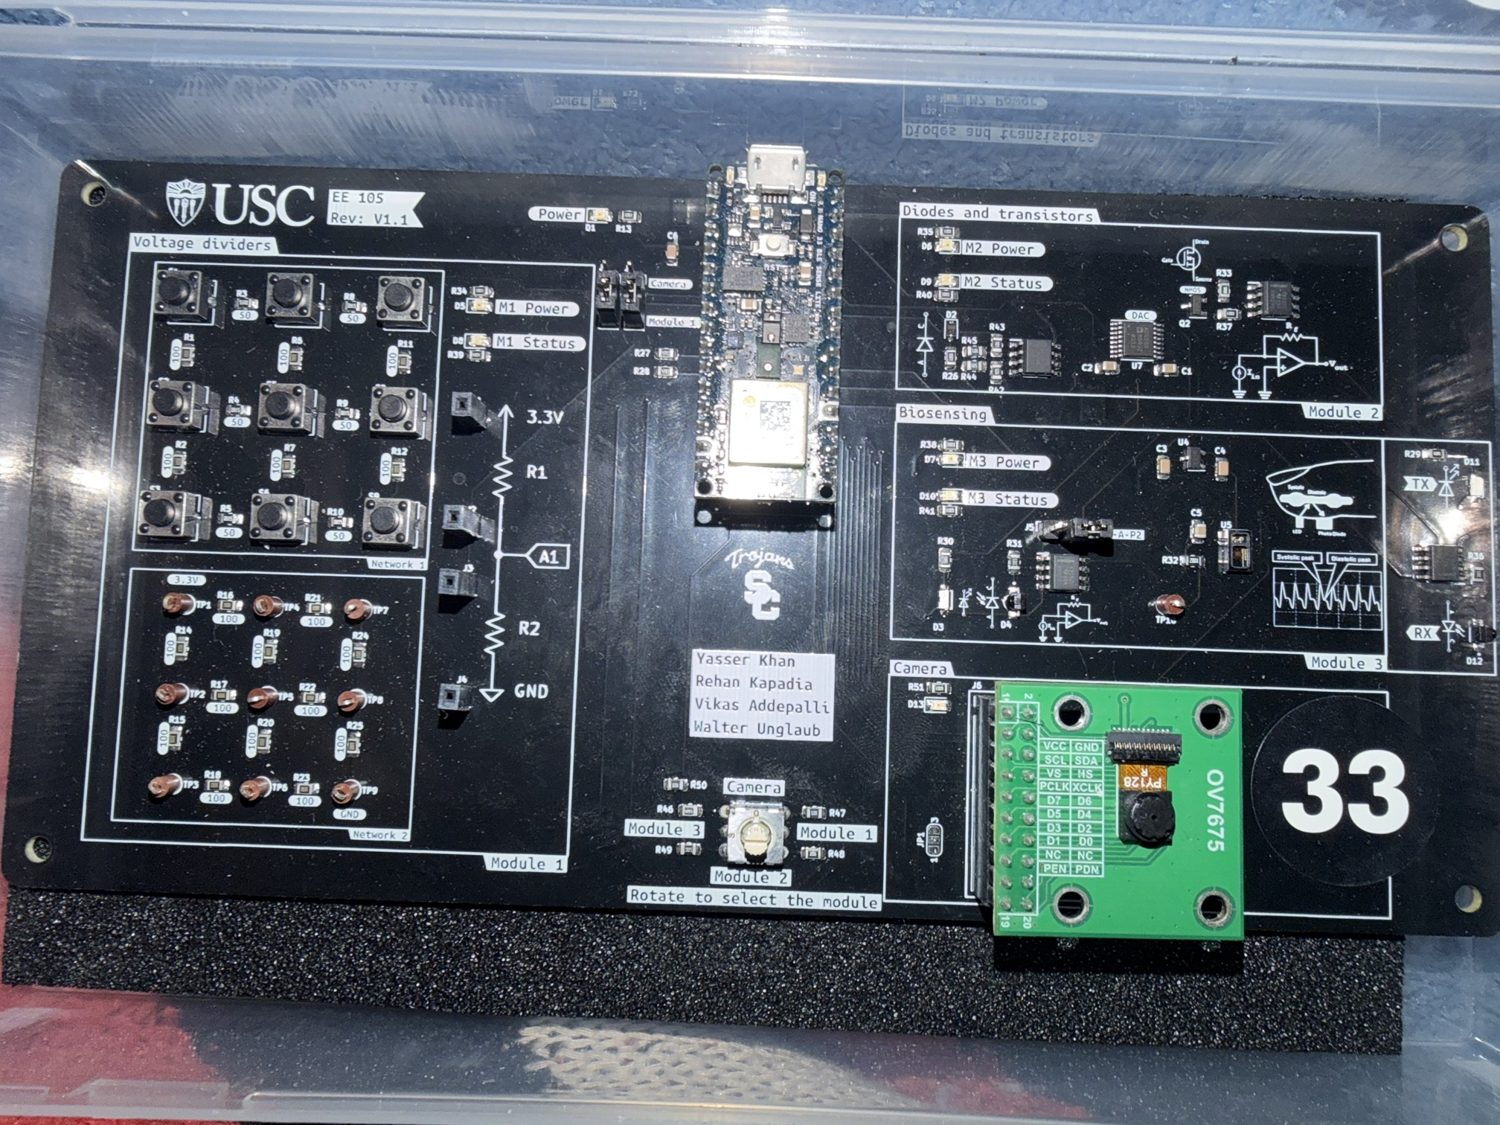
\includegraphics[width=\linewidth]{img/board.jpg}};
\begin{scope}[x={(img.south east)}, y={(img.north west)},
  lab/.style={fill=white, draw=black!70, rounded corners=1.5pt, inner sep=2.5pt, font=\sffamily\scriptsize, align=center},
  ptr/.style={-{Stealth[length=2mm]}, line width=0.9pt, white, double=black, double distance=0.5pt}]
\node[lab] (cam) at (0.86,0.07) {A\ \ camera lens};
\draw[ptr] (cam) -- (0.775,0.245);
\node[lab] (nano) at (0.78,0.955) {B\ \ Arduino Nano, with the USB socket};
\draw[ptr] (nano.west) -- (0.535,0.865);
\node[lab] (sel) at (0.42,0.07) {C\ \ module selector};
\draw[ptr] (sel) -- (0.495,0.235);
\node[lab] (jmp) at (0.22,0.955) {D\ \ two jumpers};
\draw[ptr] (jmp.south) -- (0.405,0.755);
\node[lab] (but) at (0.12,0.07) {E\ \ supported end};
\draw[ptr] (but) -- (0.10,0.30);
\end{scope}
\end{tikzpicture}
\caption{The EE\,105 board, seen from its component side. The camera~(A) looks out of the page.
The laptop is connected at the micro-USB socket of the Arduino Nano~(B). The selector~(C) must
point to \emph{Camera}. The jumpers~(D) stay as they were in the digit-recognition laboratory.
In the stand of Section~\ref{sec:stand} the board lies face down and rests on its end~(E).}
\label{fig:board}
\end{figure}

\step{Set the selector and connect the cable}
Take the board out of its box by its edges and lay it, components upwards, on a dry table of
wood or plastic. Find the rotary selector~(C in Figure~\ref{fig:board}), which is labelled
\emph{Rotate to select the module}, and turn it until its mark points to \ui{Camera}. Leave
the two small black jumpers beside the Nano~(D) where they are: they were set for the camera
during the digit-recognition laboratory. If a transparent protective film covers the camera
lens~(A), peel it off. Plug the small end of the USB cable into the socket of the Nano~(B) and
the other end into the laptop, directly and not through a hub or a docking station.
\checkpoint{A small light is lit on the board, and Windows has played its ``device connected''
sound.}

\begin{iffail}
If nothing lights up, try another USB socket of the laptop and then another cable. Many
micro-USB cables are made for charging only and carry no data; with such a cable the light
comes on, but the board never appears in the list of ports in Step~\ref{st:port}.
\end{iffail}

\subsection{Upload the sketch}

\step{Open the sketch}
In the Arduino IDE choose \menu{File}\then\menu{Open\ldots}, go to the folder
\file{C:\bs ee105\bs camera-to-latex\bs firmware\bs capture}, select \file{capture.ino} and
click \ui{Open}. The sketch appears in a new window; the empty window may be closed.

\step{Check that the sketch names the right camera}\label{st:model}
Near the top of the sketch, below the line that contains the word \emph{settings}, look for a
line that begins as follows.
\begin{filebox}{Sketch capture.ino: the first setting}
#define CAMERA_MODEL  OV7675
\end{filebox}
\checkpoint{The line is present.}
\rationale{The camera library supports two sensors and assumes the older OV7670 unless it is
told otherwise. Copies of the sketch made before 24 November 2026 lack this line and therefore
configure the board's OV7675 with the settings of the wrong sensor.}
\begin{iffail}[If the line is missing]
Your copy of the repository is out of date. Close the sketch window, carry out
Step~\ref{st:uptodate}, and open the sketch again.
\end{iffail}

\step{Select the board and the port}\label{st:port}
Choose \menu{Tools}\then\menu{Board}\then\menu{Arduino Mbed OS Nano Boards}\then\menu{Arduino
Nano 33 BLE}. (The Sense Lite has no entry of its own; it is programmed as a Nano 33 BLE.) Then
choose \menu{Tools}\then\menu{Port} and click the entry that names the board, for example
\emph{COM5 (Arduino Nano 33 BLE)}. Write the port name down.
\checkpoint{The bottom right corner of the IDE window shows \emph{Arduino Nano 33 BLE on COM}
followed by a number.}

\step{Upload}\label{st:upload}
Click the round button with the arrow that points to the right, at the top left of the window
(tooltip \ui{Upload}). The IDE first translates the sketch, which takes between two and ten
minutes the first time, and then transfers it, which takes a few seconds. During the transfer
the port may disappear and reappear, sometimes under a different number. A warning that little
memory is left may appear; it is harmless, because the sketch deliberately reserves most of the
board's memory for one picture.
\checkpoint{The IDE shows the message \emph{Done uploading}.}

\begin{iffail}[If the upload fails or never starts]
Press the small white button on the Nano twice in quick succession. An orange light on the Nano
then fades in and out, which shows that the board is waiting for a program. Select the port
again (\menu{Tools}\then\menu{Port}; its number may have changed) and click \ui{Upload} once
more.
\end{iffail}

\step{Release the port}
Close the Arduino IDE completely.
\rationale{Only one program at a time can use a serial port. As long as the IDE, or its
\emph{Serial Monitor}, holds the port, the Python programs of the following steps are refused
with the message \emph{Access is denied}.}

\subsection{Test the link between board and laptop}

The remaining steps of this task are given in the PowerShell window of Step~\ref{st:t1open}. If
that window has been closed in the meantime, carry out Step~\ref{st:t1open} again first.

\step{List the serial ports}
\begin{ps}
python -m pipeline.capture --list
\end{ps}
\begin{out}[What you should see (the port number will differ)]
COM5                     USB Serial Device (COM5)  vid=9025 pid=32858
\end{out}
\checkpoint{One line shows \texttt{vid=9025}, the identification number of Arduino. Other
lines, for example for Bluetooth devices, may appear as well.}

\step{Ask the board whether it is alive}\label{st:ping}
\begin{ps}
python -m pipeline.capture --ping
\end{ps}
\begin{out}
port COM5
board answers: 320x240, 1 byte(s) per pixel
\end{out}
\checkpoint{The second line appears within a few seconds.}

\begin{iffail}
If this is the first command since the board was plugged in, give it a second time before
drawing any conclusion: the camera needs a moment to start when the port is opened for the
first time. Otherwise the answer names the cause. \emph{Access is denied}: another program
holds the port; close the Arduino IDE. \emph{cannot pick the board's port automatically}: more than one candidate is
connected; unplug other Arduino boards, or name the port by adding it to the command, as in
\code|python -m pipeline.capture --ping --port COM5|. \emph{unexpected ping answer: ERR
camera}: the sketch runs but cannot start the camera; see Section~\ref{sec:t1trouble}.
\emph{no answer}: the sketch is not on the board; repeat Step~\ref{st:upload}.
\end{iffail}

\subsection{First pictures and orientation}

\step{Open the viewfinder}\label{st:viewfinder}
\begin{ps}
python -m pipeline.capture --series data\raw\rig --names "first"
\end{ps}
A window with the title \emph{capture series} opens and shows what the camera sees, enlarged
twofold. The yellow line at the top names the photograph that will be saved next, and the line
at the bottom lists the keys (Table~\ref{tab:serieskeys}). Three properties of this window
matter throughout Tasks~1, 2 and~4.
\begin{itemize}
\item The picture is renewed only about once per second. After moving anything, wait until the
  picture has changed and then stood still for two seconds before judging or saving it.
\item The keys act only while this window is the active one: click once on the picture first.
\item The keys are lower-case letters. If they have no effect, the \key{Caps Lock} key is on.
\end{itemize}

\begin{table}[H]
\centering
\begin{tabular}{C{2.2cm}L{8.6cm}}
\toprule
\hd{Key} & \multicolumn{1}{c}{\hd{Effect in the capture-series window}} \\
\midrule
\key{Space} & Save the current picture under the name shown, and go on to the next name \\
\key{B} & Go back one name, so that a photograph can be taken again \\
\key{N} & Skip the current name without saving \\
\key{Q} or \key{Esc} & Close the window \\
\bottomrule
\end{tabular}
\caption{Keys of the capture-series window. After the last name of its list, the window closes
by itself.}
\label{tab:serieskeys}
\end{table}

Hold the board by its edges about 15\,cm above a printed page of test lines, with the camera
looking down at the page and a lamp lighting the page, and move it until a line is in view.
\checkpoint{Printed characters can be recognized in the window, even if they are upside down,
mirrored or slightly blurred. A picture of noise or stripes, or a uniformly gray picture, is a
failure: see Section~\ref{sec:t1trouble}.}

\step{Test for a mirror image}\label{st:orient}
Turn the \emph{page} until the text in the window stands upright, and look at the letters.
\begin{itemize}
\item If they read normally, no setting is needed.
\item If they are reversed as in a mirror, the setting \code|FLIP_H| must become \code|True|.
  Press \key{Q} to close the window, change the setting as described in
  Section~\ref{sec:setting}, and repeat Step~\ref{st:viewfinder} to confirm that the text now
  reads normally.
\end{itemize}
Finally press \key{Space} to save one photograph, which also closes the window.
\checkpoint{Upright text in the viewfinder reads normally, PowerShell has printed \emph{saved
first.png}, and the file exists in the folder \file{data\bs raw\bs rig}.}

\rationale{A sensor may deliver its lines in either direction, so a mirror image cannot be
excluded in advance; it can be undone only by this setting. An image that is merely upside
down needs no setting, because the page can be turned. Photographs are stored exactly as the
camera delivers them, and the setting is applied whenever a photograph is read; a correction
made later therefore also holds for photographs taken earlier.}

\subsection{The soak test}

\step{Request one hundred pictures}\label{st:soak}
Lay the board, components upwards, on the wooden or plastic table, with a lit page or wall in
front of the camera, and run:
\begin{ps}
python -m pipeline.capture --soak 100
\end{ps}
The command requests 100 pictures in succession and verifies each one by its \term{checksum},
the sum of all its pixel values, which the board transmits after the pixels. It runs for two to
four minutes.
\begin{out}[What you should see (the measured values will differ)]
port COM5
first frame 320x240, mean level 121
100/100 frames OK, 0 failed, 1.31 s per frame
\end{out}
\checkpoint{The last line begins with \texttt{100/100 frames OK}. Enter the time per frame in
the record.}

\begin{iffail}[If some pictures fail]
Each failure is reported on a line of its own with its reason (\emph{timeout} or \emph{checksum
mismatch}). Connect the board to a socket of the laptop itself, use a shorter cable, and repeat
the test. The application repeats a failed request up to three times, so that one or two
failures in a hundred do not prevent further work; the criterion of this task, however, is a
clean run. If failures persist, enter their number in the record and inform the lead.
\end{iffail}

\subsection{Build the stand}
\label{sec:stand}

\subsubsection*{Requirements}

Any construction is acceptable that meets the following five requirements.
\begin{enumerate}
\item The lens looks straight down at the desk from a height of 16 to 18\,cm, and stays there
  when the cable or the page is touched.
\item Around the point of the desk directly below the lens, at least 20\,cm are free in every
  direction, so that a printed page can be moved to bring any of its lines below the lens.
\item The page can lie at two distances from the lens: on the desk, and on a firm platform 5 to
  7\,cm thick.
\item Nothing conductive touches the board, and nothing presses on the camera or on the Nano.
\item The USB cable is fastened to the stand, so that a pull on the cable cannot move the
  board.
\end{enumerate}
The camera is fixed and the \emph{page} is raised for close work, because a platform of books is
easier to rebuild exactly than a stand of adjustable height.

\subsubsection*{A construction from books}

Figure~\ref{fig:stand} shows a stand that needs only books, two cloths and tape. A large
hardcover book projects from a stack like an arm, and the board lies face down on the end of
the arm.

\begin{figure}[H]
\centering
\begin{tikzpicture}[x=0.22cm, y=0.22cm, font=\scriptsize, >={Stealth[length=1.6mm]}]
% desk
\draw[line width=0.9pt] (-1,0) -- (52.5,0);
% base stack
\fill[black!14] (0,0) rectangle (18,14); \draw (0,0) rectangle (18,14);
\foreach \y in {2.8,5.6,8.4,11.2} \draw[black!45] (0,\y) -- (18,\y);
% arm
\fill[black!32] (3,14) rectangle (31,17); \draw (3,14) rectangle (31,17);
% weights on the arm
\fill[black!14] (3,17) rectangle (16.5,23); \draw (3,17) rectangle (16.5,23);
\foreach \y in {19,21} \draw[black!45] (3,\y) -- (16.5,\y);
% cloth, board, cloth, light weight
\fill[black!60] (25.6,17) rectangle (31,17.45);
\fill[green!40!black] (26,17.45) rectangle (43.5,17.8);
\fill[black!60] (25.6,17.8) rectangle (31,18.25);
\fill[black!14] (25.9,18.25) rectangle (30.7,20.6); \draw (25.9,18.25) rectangle (30.7,20.6);
% camera
\fill[black] (38.6,16.75) rectangle (40.4,17.45);
\fill[black] (39.2,16.3) rectangle (39.8,16.75);
% platform and pages
\fill[black!7] (30.5,0) rectangle (48.5,5.6); \draw[densely dashed] (30.5,0) rectangle (48.5,5.6);
\draw[line width=1.3pt] (31.5,5.75) -- (47.5,5.75);
\draw[line width=1.3pt, black!55] (29.5,0.15) -- (49.5,0.15);
% view
\draw[densely dotted, line width=0.6pt] (39.5,16.3) -- (31.6,0.15);
\draw[densely dotted, line width=0.6pt] (39.5,16.3) -- (47.4,0.15);
% dimensions
\draw[<->] (50.6,0) -- (50.6,16.3);
\draw[black!55] (39.9,16.3) -- (50.9,16.3);
\node[anchor=west, align=left] at (50.7,10.4) {16 to\\18\,cm};
\draw[<->] (44.9,5.75) -- (44.9,16.3);
\node[anchor=west, align=left] at (45.0,12.6) {about\\11\,cm};
\draw[<->] (18,9.3) -- (39.5,9.3);
\draw[black!55, densely dashed] (39.5,16.2) -- (39.5,6.2);
\node[anchor=south] at (27.6,9.3) {20\,cm or more};
% labels
\node[align=center] at (9,7) {base stack};
\node[align=center] at (9.7,20.1) {heavy books};
\node[anchor=west] at (4,15.5) {arm: a large hardcover book};
\node[anchor=south, align=center] (bl) at (36.8,20.6) {board, face down,\\between two cloths};
\draw[->] (bl.south) -- (35.3,18.0);
\node[anchor=south, align=center] (wl) at (25.5,23.4) {light book};
\draw[->] (wl.south) -- (28.2,20.8);
\node[anchor=north, align=center] (cl) at (35.2,14.9) {lens};
\draw[->] (cl.east) -- (39.0,16.4);
\node[anchor=north, align=center] at (39.5,-0.4) {platform (for lines only), page on top};
\node[anchor=north, align=center] at (9,-0.4) {desk};
\end{tikzpicture}
\caption{Side view of a stand built from books. For the symbol sheets the page lies on the desk,
16 to 18\,cm below the lens (\emph{sheet position}). For the test lines the page lies on a
platform that brings it to about 11\,cm below the lens (\emph{line position}). The dotted lines
show the camera's view.}
\label{fig:stand}
\end{figure}

\step{Build the stack and the arm}
On a desk, stack books to a height of about 14\,cm, with one straight vertical face. Lay a large
hardcover book, the \emph{arm}, on top, so that it projects 12 to 15\,cm beyond that face, and
lay two or three heavy books on the part of the arm that rests on the stack.
\checkpoint{The projecting end of the arm does not sink or rock when it is pressed down gently
with a finger, and its upper surface is 17 to 18\,cm above the desk.}

\step{Place the board}
Unplug the USB cable from the laptop. Lay a folded dry cloth on the projecting end of the arm.
Turn the board over and lay it on the cloth with its components downwards and its long side in
line with the arm, so that the end marked~E in Figure~\ref{fig:board} rests on the arm over a
length of 4 to 5\,cm and the rest of the board, with the Nano and the camera, projects freely
beyond the arm. Lay the second folded cloth on the supported end and a paperback book on it.
\checkpoint{Seen from the side, the board is level, and nothing touches the camera or the Nano.
Stand the ruler on the desk beside the camera: the front of the lens is between 16 and 18\,cm
above the desk. Add or remove a thin book of the base stack to correct the height.}

\step{Fasten the cable}
Plug the cable into the laptop again. Lead it from the Nano back along the arm, leaving a loose
bend of a few centimetres at the plug, and tape it to the arm.
\checkpoint{A gentle pull on the cable beyond the tape does not move the board.}

\step{Place a white background and the lamp}
Lay two blank white sheets on the desk below the camera, so that the camera sees only white
paper wherever no printed page lies. Place the lamp, or better two lamps, to the left and to
the right of the board at a distance of 30 to 40\,cm, with their heads no higher than the
board, so that the light falls on the paper at a shallow angle from the side.
\begin{ps}
python -m pipeline.capture --series data\raw\rig --names "blank"
\end{ps}
Look at the viewfinder. The picture should be an even light gray. A darker region with a sharp
border is the shadow of the board, of the cable or of the arm: move the lamp until it has left
the picture. A white spot is the reflection of the lamp: lower the lamp or move it farther to
the side. Then press \key{Space}.
\checkpoint{The viewfinder shows an evenly lit, empty sheet, without shadows and without bright
spots, and \emph{saved blank.png} has been printed.}

\step{Find the direction of the page}\label{st:pagedir}
\begin{ps}
python -m pipeline.capture --series data\raw\rig --names "direction"
\end{ps}
Lay page~1 of the printed test lines below the camera and turn it in steps of a quarter turn
until its text stands upright in the viewfinder and runs from left to right. Stick a strip of
tape on the desk and draw on it an arrow that points towards the top edge of the page as it now
lies. Press \key{Space}.
\checkpoint{The arrow on the desk shows where the top of every page must point from now on.}

\subsection{Calibrate the two positions}

\subsubsection*{Geometry}

The calibration measures the \term{scale} $s$ of a photograph, the number of pixels that one
centimetre of paper occupies. The scale follows from the distance $d$ between the lens and the
page. A lens with a horizontal angle of view $\theta$ sees a strip of paper of width
\[
  w = 2\,d\,\tan\frac{\theta}{2} = k\,d ,
\]
and this strip is spread over the 320 pixels of the long side of the picture, so that
\[
  s = \frac{320}{w} = \frac{320}{k\,d} .
\]
A printed length $\ell$ then appears with $\ell\,s$ pixels. For the lens of this board the
published angles of view give a constant $k$ between 0.89 and 1.0. Two printed lengths matter:
the height of a capital letter, 0.96\,cm at the print size of 40\,pt, and the width of the
widest test line, T39, which is 9.67\,cm. Table~\ref{tab:geometry} lists what the formula
predicts for them; the calibration replaces these predictions by measurements.

\begin{table}[H]
\centering
\begin{tabular}{C{1.7cm}C{2.5cm}C{2.2cm}C{2.0cm}C{2.0cm}}
\toprule
\hd{Distance $d$} & \hd{Width in view $w$} & \hd{Scale $s$} & \hd{Capital height} & \hd{Width of T39} \\
\midrule
17 cm & 15.1--17.0 cm & 19--21 px/cm & 18--20 px & 182--205 px \\
15 cm & 13.4--15.0 cm & 21--24 px/cm & 20--23 px & 206--232 px \\
13 cm & 11.6--13.0 cm & 25--28 px/cm & 24--27 px & 238--267 px \\
12 cm & 10.7--12.0 cm & 27--30 px/cm & 26--29 px & 258--290 px \\
11 cm & 9.8--11.0 cm & 29--33 px/cm & 28--31 px & 281--316 px \\
10 cm & 8.9--10.0 cm & 32--36 px/cm & 31--35 px & 309--348 px \\
\bottomrule
\end{tabular}
\caption{Predicted size of printed material in the photograph, for material printed at 40\,pt.
The depth of the view is three quarters of its width.}
\label{tab:geometry}
\end{table}

Two requirements fix the two positions. A block of the symbol sheets measures $12.7 \times
10.0$\,cm including its corner squares; to show it whole, the view must be at least
$13.5 \times 10.8$\,cm, which the table places at a distance of 16 to 18\,cm. This is the
\emph{sheet position}. For the test lines, larger letters are read more reliably. In simulated
photographs read with the fallback classifier, 57 of the 80 lines were read exactly when
capitals were 24 pixels tall, 63 at 28 pixels and 65 at 30 pixels; of the nine lines of plain
text, one, four and six. The picture, however, is only 320 pixels wide, and line T39 is 10.1
capital heights long: it occupies 282 pixels when capitals are 28 pixels tall and 302 pixels
when they are 30. The \emph{line position} is therefore the distance at which line T39 is
between 280 and 300 pixels wide, which corresponds to a scale of 29 to 31\,px/cm and to
capitals of 28 to 30 pixels; the table places it at 11 to 12\,cm. (The update report named a
provisional height of about 12.5\,cm and capitals of 30 pixels or more. The analysis above
refines both figures: at 12.5\,cm capitals would measure only 25 to 28 pixels, and above 30
pixels line T39 no longer fits into the picture.)

\subsubsection*{The sheet position}

\step{Photograph a ruler and a block on the desk}\label{st:calsheet}
\begin{ps}
python -m pipeline.capture --series data\raw\rig --names "desk_ruler,A1_0"
\end{ps}
For the first photograph, lay the ruler on the white sheet below the camera, parallel to the
long side of the picture, so that its centimetre scale crosses the whole picture; press
\key{Space}. For the second, remove the ruler and lay page~1 of the printed symbol sheets on the
desk, its top towards the arrow, so that its upper block is in the middle of the picture. The
small words below each block give its name; this one is block~A1. Cover the lower block of the
page with a blank sheet whose edge runs through the middle of the white gap between the two
blocks. Check in the viewfinder that all four corner squares are inside the picture, that the
hollow square is at the top left, and that white paper is visible between each square and the
border of the picture; then press \key{Space}.
\checkpoint{PowerShell has printed \emph{saved desk\_ruler.png} and \emph{saved A1\_0.png}.}

\begin{iffail}[If the four corner squares do not fit into the picture]
The camera is too low. Add a thin book to the base stack and repeat this step. If, on the
contrary, the block occupies less than three quarters of the width of the picture, the camera is
higher than necessary: remove a book.
\end{iffail}

\step{Measure the scale on the desk}\label{st:paint}
\begin{ps}
mspaint data\raw\rig\desk_ruler.png
\end{ps}
The photograph opens in Paint. Enlarge it with the slider at the bottom right of the window
until the centimetre marks can be told apart. Rest the tip of the pointer on the mark of 2\,cm
and read the two numbers at the bottom left of the window: they are the position of the
pointer in pixels, counted from the left and from the top of the photograph. Note the first
number, $x_1$. Do the same on the mark of 12\,cm for $x_2$. The scale on the desk is
\[
  s_{\text{desk}} = \frac{x_2 - x_1}{10\ \text{cm}} .
\]
For example, positions of 41 and 243 give a scale of 20.2\,px/cm and a view that is
$320/20.2 = 15.8$\,cm wide. Close Paint without saving. (Paint shows the photograph as it is
stored. If the setting \code|FLIP_H| is \code|True|, the stored photograph is the mirror image
of what the viewfinder showed; distances between marks are not affected.)
\checkpoint{The scale is between 18 and 23\,px/cm. Enter it in the record.}

\begin{iffail}[If Paint does not open the photograph]
Open the folder with the command \code|explorer data\raw\rig|, right-click the file
\file{desk\_ruler.png} and choose \menu{Open with}\then\menu{Paint}.
\end{iffail}

\step{Let the cropping program judge the block}\label{st:calcrop}
\begin{ps}
python -m tools.crop_sheet --photos data\raw\rig --out data\raw\rig\crops
\end{ps}
\begin{out}[What you should see (the number of pixels will differ)]
A1_0.png: 35 crops, capitals 20 px

35 crops from 1 photos -> data\raw\rig\crops
\end{out}
\checkpoint{The line for \file{A1\_0.png} reports 35 crops; the words \emph{read as an upright
page} may follow and are acceptable. The stand is now at a usable sheet position. Measure the
height of the lens above the desk once more and enter it in the record.}

\begin{iffail}
The word \emph{skipped}, followed by a reason in parentheses, means that the program did not
find the four corner squares. Repeat Step~\ref{st:calsheet} with more white paper around the
block, with the page lying flat, and without a shadow on any corner.
\end{iffail}

\subsubsection*{The line position}

\step{Build the platform and photograph line T39}\label{st:calline}
Lay flat books below the camera to a height of 6\,cm, with a blank white sheet on top. This is
the \emph{platform}. Lay page~8 of the printed test lines on it, its top towards the arrow; the
names of the lines are printed small at the right margin of the page.
\begin{ps}
python -m pipeline.capture --series data\raw\rig --names "p1_T39"
\end{ps}
Move the page until line T39, $y=ax^{2}+bx+c$, lies in the middle of the picture, with equal
white margins to its left and right. Parts of the lines above and below it may show at the
upper and lower borders of the picture; they do no harm and are not to be covered. Press
\key{Space}.
\checkpoint{\emph{saved p1\_T39.png} has been printed.}

\rationale{The program keeps only the row of ink nearest the middle of the picture. In 240
simulated photographs, the number of lines read exactly was the same, 196, whether the
neighbouring lines of the page were present or not; an aim that was 7\,mm too high or too low
changed it by at most two.}

\step{Measure the width of the line}\label{st:measure}
\begin{ps}
mspaint data\raw\rig\p1_T39.png
\end{ps}
Enlarge the picture as far as the slider allows. Rest the pointer on the leftmost dark pixel of
the line and note the first number at the bottom left, $x_{\text{left}}$. Rest it on the
rightmost dark pixel of the line and note $x_{\text{right}}$. Then
\[
  W = x_{\text{right}} - x_{\text{left}} + 1, \qquad
  s_{\text{line}} = \frac{W}{9.67\ \text{cm}}, \qquad
  h \approx \frac{W}{10} ,
\]
where $W$ is the width of the line, $s_{\text{line}}$ the scale and $h$ the height of a capital
letter, all in pixels. The white margins of the line are $x_{\text{left}}$ on the left and
$319 - x_{\text{right}}$ on the right. While the picture is enlarged, judge its sharpness: the
two bars of the equals sign must be separated by a clearly lighter row of pixels, and the small
2 must be recognizable as a 2. Close Paint without saving.
\checkpoint{$W$, the two margins and the verdict on sharpness are entered in the first row of
Table~\ref{tab:trials}.}

\begin{table}[H]
\centering
\begin{tabular}{C{1.3cm}C{2.3cm}C{1.9cm}C{2.3cm}C{2.5cm}}
\toprule
\hd{Trial} & \hd{Platform} & \hd{Width $W$} & \hd{Margins} & \hd{Sharp?} \\
\midrule
p1 & \hfill cm & \hfill px & \hfill px & \cbox\ yes\quad\cbox\ no \\
p2 & \hfill cm & \hfill px & \hfill px & \cbox\ yes\quad\cbox\ no \\
p3 & \hfill cm & \hfill px & \hfill px & \cbox\ yes\quad\cbox\ no \\
p4 & \hfill cm & \hfill px & \hfill px & \cbox\ yes\quad\cbox\ no \\
\bottomrule
\end{tabular}
\caption{Trials of the line position. The platform is described by its thickness.}
\label{tab:trials}
\end{table}

\step{Adjust the platform until the criteria are met}\label{st:adjust}
The criteria are: $W$ from 280 to 300 pixels; both margins at least 10 pixels; a sharp picture.
Because the size of the image is inversely proportional to the distance, a small change
$\Delta d$ of the distance changes the width by
\[
  \Delta W \approx -\,\frac{W}{d}\,\Delta d ,
\]
which near the target amounts to about 10 pixels for every 4\,mm. If $W$ is below 280, raise
the platform by 4\,mm, the thickness of a thin notebook or magazine, for every 10 pixels that
are missing; if it is above 300, lower it likewise. Then photograph and measure again under a
new name, so that the earlier photographs are kept for comparison:
\begin{ps}[Second trial]
python -m pipeline.capture --series data\raw\rig --names "p2_T39"
\end{ps}
\begin{ps}[To measure the second trial]
mspaint data\raw\rig\p2_T39.png
\end{ps}
For a third and a fourth trial, write \code|p3_T39| and \code|p4_T39| in place of
\code|p2_T39| in both commands.
\checkpoint{One trial meets all three criteria. Its platform is the \emph{line platform}: keep
its books together, mark the pile, and outline its position on the desk with tape so that it
can be put back exactly.}

\begin{iffail}[If the picture is blurred at 280 pixels but sharp when the page lies lower]
The lens cannot focus at so short a distance. Find the thickest platform at which the picture
is sharp, and enlarge the print instead of approaching it: carry out
Section~\ref{sec:bigprint} before anything is photographed for Tasks~2 and~4.
\end{iffail}

\subsection{Acceptance test with the application}

\step{Read five probe lines through the complete pipeline}\label{st:accept}
With the line platform in place, start the application:
\begin{ps}
python -m pipeline.main --new
\end{ps}
After up to half a minute, a window with the title \emph{camera to latex} shows the live
picture;
below it, two lines of text give the state of the program and its keys. Bring one of the lines
of Table~\ref{tab:probes} into the middle of the picture, wait until the picture stands still,
and press \key{Space}. The picture freezes. A box is drawn around every symbol that was found:
green where the classifier is confident, red where it is not, blue for the bar of a fraction.
The name that the classifier gives each symbol is written above its box, and the reading of the
whole line appears below the picture and in the PowerShell window. Press \key{R} to return to
the live picture. Do this for the five lines of the table, then press \key{Q}.

\begin{table}[H]
\centering
\begin{tabular}{C{1.4cm}C{3.9cm}C{1.5cm}C{3.6cm}}
\toprule
\hd{Line} & \hd{Printed content} & \hd{Page} & \hd{One box per symbol?} \\
\midrule
D03 & USC Trojans & 13 & \cbox\ yes\quad\cbox\ no \\
D08 & $z=x+iy$ & 14 & \cbox\ yes\quad\cbox\ no \\
D05 & $a^{2}+b^{2}=c^{2}$ & 13 & \cbox\ yes\quad\cbox\ no \\
D14 & $\dfrac{1}{3}+\dfrac{2}{3}=1$ & 15 & \cbox\ yes\quad\cbox\ no \\[6pt]
T39 & $y=ax^{2}+bx+c$ & 8 & \cbox\ yes\quad\cbox\ no \\
\bottomrule
\end{tabular}
\caption{Probe lines for the acceptance test of the stand. The pages are those of the printed
test lines.}
\label{tab:probes}
\end{table}

\checkpoint{For at least four of the five lines, every printed symbol has exactly one box (a
letter with a dot, an equals sign and a fraction bar each count as one symbol), the note
\emph{ink touches the photo edge} does not appear below the picture, and the reading appears
within five seconds of the key press. Whether each symbol is also \emph{named} correctly is not
judged here; that is the subject of Tasks~2 and~3.}

\begin{iffail}
Boxes that split one letter into two, or join two letters into one, on most lines indicate
letters that are too small or too blurred: review the trials of Table~\ref{tab:trials}. The
note about the photo edge means that the line was not wholly inside the picture: centre it and
read it again.
\end{iffail}

\subsection{Record and share}
\label{sec:t1record}

\step{Fill in the record}
\begin{table}[H]
\centering
\begin{tabular}{L{7.0cm}C{4.2cm}}
\toprule
\multicolumn{1}{c}{\hd{Quantity}} & \hd{Value} \\
\midrule
Board number (white disc beside the camera); date & \\
Serial port & \\
Soak test: pictures received of 100; time per picture & \\
Setting \texttt{FLIP\_H} (True or False) & \\
Height of the lens above the desk & \hfill cm \\
Scale on the desk, $s_{\text{desk}}$ & \hfill px/cm \\
Capital height reported by the cropping program & \hfill px \\
Thickness of the line platform & \hfill cm \\
Distance from the lens to the page on the platform & \hfill cm \\
Width $W$ of line T39 on the platform & \hfill px \\
Scale on the platform, $s_{\text{line}} = W / 9.67$\,cm & \hfill px/cm \\
Capital height on the platform, $h \approx W/10$ & \hfill px \\
Print size of the test lines & 40 pt \\
Probe lines with one box per symbol & \hfill of 5 \\
\bottomrule
\end{tabular}
\caption{Record of Task 1. The final report quotes these values.}
\label{tab:t1record}
\end{table}

\step{Photograph the stand}
Take a photograph of the finished stand with a telephone, from the side, with the ruler standing
beside the camera, and place it in the team's shared folder. The final report needs it, and it
allows the stand to be rebuilt.

\step{Share the orientation setting, if it was changed}
If Step~\ref{st:orient} changed \file{config.py}, record the change for the team with the
following three commands. If it did not, skip this step.
\begin{ps}
git add config.py
\end{ps}
\begin{ps}
git commit -m "Set camera orientation for the stand"
\end{ps}
\begin{ps}
git push
\end{ps}
\checkpoint{The output of the last command ends with a line that contains \texttt{main ->
main}.}

\subsection{Contingency: larger print}
\label{sec:bigprint}

This subsection is carried out only if the calibration has shown that the lens cannot give a
sharp picture in which line T39 is 280 pixels wide. The remedy is to print the test lines at
48\,pt in place of 40\,pt. Every letter is then one fifth larger, so that the same size in
pixels is reached from a distance one fifth greater, where the lens is sharper.

\step{Produce and print the larger test lines}
\begin{ps}
python -m tools.make_test_lines --pdf --font-pt 48
\end{ps}
\begin{out}
C:\ee105\camera-to-latex\test_set\test_lines.pdf: 80 lines at 48 pt, 4 per page
\end{out}
Print the new \file{test\_lines.pdf} (20 pages) at 100\,\% and discard the old print. The pages
now hold four lines each, so that the page numbers given in this document no longer apply; the
name at the right margin identifies each line. Line T39 is now 11.6\,cm long.
\checkpoint{The answer ends with \emph{4 per page}, and on paper line T39 measures 11.6\,cm.}

\step{Repeat the calibration of the line position}
Repeat Steps~\ref{st:calline} to~\ref{st:adjust} with a thinner platform, beginning at 3.5\,cm.
The criteria in pixels are unchanged: $W$ from 280 to 300, margins of at least 10, a sharp
picture. In the record, the scale is now $s_{\text{line}} = W / 11.6$\,cm, and the print size
is 48\,pt.

\step{Share the new print}
\begin{ps}
git add test_set\test_lines.pdf
\end{ps}
\begin{ps}
git commit -m "Print the test lines at 48 pt"
\end{ps}
\begin{ps}
git push
\end{ps}

\subsection{If something goes wrong}
\label{sec:t1trouble}

\trouble{The board does not appear under \menu{Tools}\then\menu{Port}, or in the list of
serial ports}
\cause The cable carries no data, or the driver was not installed.
\remedy Use another cable. Open the Arduino IDE once more and accept the installation of the
device software; then unplug the board and plug it in again.

\trouble{\texttt{could not open port 'COM5': PermissionError \ldots{} Access is denied}}
\cause Another program holds the port: the Arduino IDE, its Serial Monitor, or a second
PowerShell window in which a capture command is still running.
\remedy Close that program or window.

\trouble{\texttt{ERR camera} in an answer, or in red letters in the viewfinder}
\cause The sketch could not start the camera.
\remedy Check that the selector points to \emph{Camera} and that the green camera module sits
firmly on its pins; unplug the USB cable and plug it in again. If the message remains, confirm
Step~\ref{st:model} and upload the sketch again. If it still remains, compare the two
jumpers~(D in Figure~\ref{fig:board}) with the handout of the digit-recognition laboratory, or
ask the teaching staff, before moving them.

\trouble{\texttt{timeout waiting for frame header}, or \texttt{no answer to b'p'}}
\cause The board runs a different sketch, or has stopped.
\remedy Unplug the cable and plug it in again, then repeat Step~\ref{st:ping}. If it fails
again, repeat Step~\ref{st:upload}.

\trouble{The picture is noise, diagonal stripes or a negative}
\cause The camera and the sketch disagree about the format of the pixels.
\remedy First confirm Step~\ref{st:model}. If that line is present, open the sketch in the
Arduino IDE, change the line \code|#define USE_GRAYSCALE 1| to \code|#define USE_GRAYSCALE 0|,
upload, and look again. If the picture is still wrong, also change \code|#define Y_OFFSET 0|
to \code|#define Y_OFFSET 1| and upload once more. To learn whether the transfer itself is at
fault, change \code|#define TEST_PATTERN 0| to \code|#define TEST_PATTERN 1|: the camera then
sends vertical bars in place of the scene, and clean, straight bars prove that the transfer
works. Set it back to 0 afterwards.

\trouble{The picture is uniformly dark or uniformly bright}
\cause The protective film is still on the lens, the lens is covered, or the lamp shines into
the lens.
\remedy Remove the film; light the page, not the camera. The camera adjusts its exposure by
itself during the first pictures after a command has started, so wait for several pictures.

\trouble{The picture is recognizable but blurred at every distance}
\cause The lens is dirty.
\remedy Breathe on the lens and wipe it gently with a clean, soft cloth. Do not turn the lens.

\trouble{The viewfinder does not react to keys}
\cause Another window is active, or \key{Caps Lock} is on.
\remedy Click once on the picture, switch \key{Caps Lock} off, and press the key again.

\section{Task 2: The symbol sheets and the retraining of the classifier}
\sectionmark{Task 2: Symbol sheets and retraining}
\label{sec:t2}

\subsection{Purpose, conditions and criterion}

\begin{plain}{Task 2 at a glance}
\textbf{Purpose.} The classifier of the quick start has learned from synthetic drawings only: it
has never seen a photograph taken by the board. In this task every symbol is photographed
through the real lens. The 18 blocks of the symbol sheets are photographed three times each,
the 54 photographs are cut into 1{,}890 labelled images of single symbols (\term{crops}), and
the network is trained again on the synthetic and the real images together. Crops from
photographs that the training never sees then measure the accuracy of the classifier on real
symbols, for which the project's target is 95\,\%.

\textbf{Before you begin.} Task~1 is complete: the stand is at its sheet position, the
orientation is settled, and the nine printed sheet pages are at hand. The quick start of the
Set-up Guide has been completed on this laptop with the neural network, so that the synthetic
training set and the file \file{models\bs symbols\_v1.keras} exist. The laptop is connected
to its charger.

\textbf{Complete when.} (1)~All 54 photographs have been cropped, none was skipped, and every
debug picture has been inspected. (2)~The network has been retrained, and its accuracy on the
held-out real crops is recorded. (3)~The retrained classifier reads the simulated test lines
no worse than the old one. (4)~The classifier has been uploaded for the team, and the
photographs are stored in the team's shared folder.

\textbf{Time.} About 45 minutes of photography, 20 minutes of cropping and inspection, about
one hour of unattended training, and 20 minutes of evaluation and upload.
\end{plain}

\subsection{What is being photographed}

\begin{figure}[H]
\centering
\begin{minipage}[c]{0.36\linewidth}\centering
\fbox{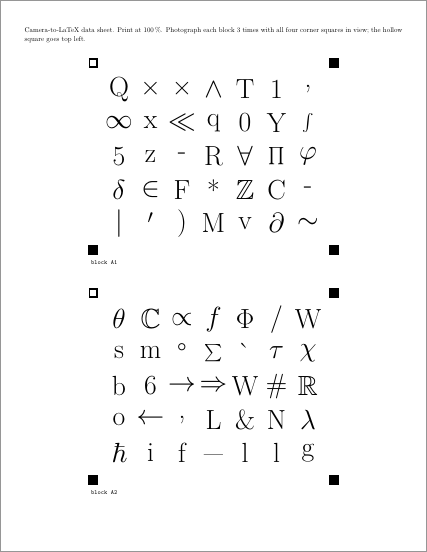
\includegraphics[width=0.95\linewidth]{img/sheet_page.png}}
\end{minipage}\hfill
\begin{minipage}[c]{0.60\linewidth}\centering
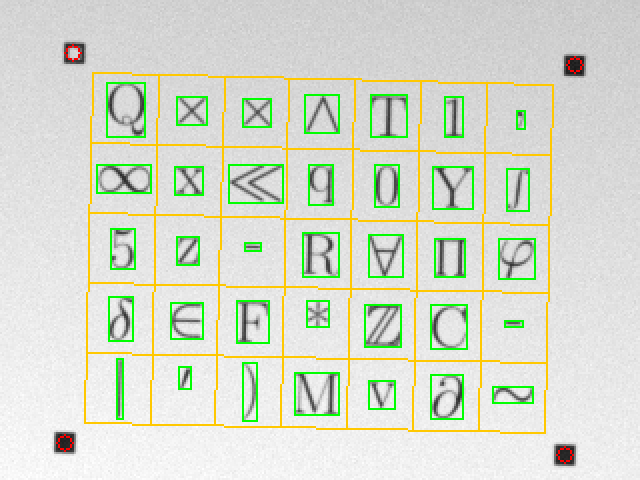
\includegraphics[width=\linewidth]{img/sheet_debug.png}
\end{minipage}
\caption{Left: page~1 of the symbol sheets, with the blocks A1 and A2. Right: a simulated
photograph of block~A1 as the cropping program marks it for inspection: a circle on each corner
square, the grid of cells, and a box around the ink found in each cell.}
\label{fig:sheet}
\end{figure}

Each of the nine pages carries two \term{blocks}. A block is a grid of 35 symbols in five rows
of seven, with a small square at each of its four corners (Figure~\ref{fig:sheet}). Three of the
squares are filled and one, at the top left, is hollow. The cropping program finds the grid by
these squares, and it knows from the file \file{sheets\bs layout.json} which symbol was printed
in which cell, so that every piece of ink it cuts out receives its correct label without
anybody typing it. The name of a block is printed in small type below it. The eighteen blocks
form three sets of six: in the blocks A1 to A6 the letters are upright, as in text; in B1 to B6
they are italic, as in formulas; C1 to C6 mix the two. Together the three sets contain each of
the 182 symbols at least three times, and symbols that are easily confused more often.

Each block is photographed three times, with small changes between the photographs, because the
classifier should learn the symbol and not one particular photograph of it. The photographs of
block~A1 are named \file{A1\_1}, \file{A1\_2} and \file{A1\_3}; the list of all 54 names, in
the order of the printed pages, is the file \file{sheets\bs photo\_names.txt}.

\subsection{Photograph the eighteen blocks}

\step{Prepare the stand}
Remove the line platform, so that pages lie on the desk at the sheet position. Check that the
blank white sheets still cover the desk below the camera and that the lamps stand as in Task~1.
\checkpoint{The desk below the camera is white and evenly lit.}

\step{Open the project in PowerShell}
% The opening sequence, written out in full. Input wherever a task may begin in a new window.
If a PowerShell window whose prompt begins with \texttt{(.venv)} is still open, use it and go
on to the next step. Otherwise open a new window (click \ui{Start}, type \code|powershell|,
click \ui{Windows PowerShell}) and give the two commands of the opening sequence in it.
\begin{ps}[Opening sequence, command 1 of 2]
cd C:\ee105\camera-to-latex
\end{ps}
\begin{ps}[Opening sequence, command 2 of 2]
.\.venv\Scripts\Activate.ps1
\end{ps}
\checkpoint{The prompt reads:}
\venvprompt


\step{Start the series}\label{st:sheetseries}
\begin{ps}
python -m pipeline.capture --series data\sheets --names-file sheets\photo_names.txt
\end{ps}
The viewfinder of Task~1 opens. Its yellow line reads \emph{1/54\ \ next: A1\_1}: the first of
54 photographs will be saved as \file{A1\_1.png}.
\checkpoint{The viewfinder shows the live picture and the name \emph{A1\_1}.}

\step{Photograph one block three times}\label{st:oneblock}
For each block, in the order in which the viewfinder asks for them:
\begin{enumerate}
\item Lay the page on the desk, its top towards the arrow, with the block named in the
  viewfinder in the middle of the picture. Cover the other block of the page with a blank sheet
  whose edge runs through the middle of the white gap between the two blocks.
\item Check four things in the viewfinder: all four corner squares are inside the picture;
  white paper is visible between each square and the border of the picture; the hollow square
  is at the top left; and no shadow or bright spot lies on the block.
\item Wait until the picture has stood still for two seconds, and press \key{Space}. PowerShell
  prints \emph{saved A1\_1.png}, and the viewfinder asks for \emph{A1\_2}.
\item Push the page about half a centimetre to one side and turn it very slightly, so that its
  edge is no longer exactly parallel to the border of the picture. Check the four things again,
  wait, and press \key{Space}.
\item Push the page half a centimetre the other way, and change the light a little: move one
  lamp by a hand's width, or shade it partly with a sheet of paper. Check, wait, and press
  \key{Space}.
\end{enumerate}
Then go on to the next block. The lower block of a page follows its upper block; move the blank
sheet onto the block that has just been photographed.
\checkpoint{After the 54th photograph the viewfinder closes by itself.}

\begin{note}[Mistakes and interruptions]
If you pressed \key{Space} too early, press \key{B}: the viewfinder goes back one name, and the
next \key{Space} replaces the faulty photograph. The series may be interrupted at any time with
\key{Q}. When the command of Step~\ref{st:sheetseries} is given again, it begins once more at
\emph{A1\_1}; names that already have a photograph are marked \emph{(exists)}, and \key{N}
passes over them one at a time without saving.
\end{note}

\begin{caution}[The page must not be turned]
A page that is photographed upside down is recognized only if the hole of its hollow square is
visible in the photograph, and at this distance the hole is only a few pixels wide. If
the hole cannot be made out, the program takes the page to be upright; a page that was in fact
turned would then give every one of its 35 crops the label of another symbol, and the
classifier would be trained on false examples. Always lay the page with its top towards the
arrow.
\end{caution}

\step{Count the photographs}
\begin{ps}
(Get-ChildItem data\sheets -Filter *.png).Count
\end{ps}
\checkpoint{The answer is \texttt{54}.}

\subsection{Cut the photographs into crops}

\step{Run the cropping program}\label{st:crop}
\begin{ps}
python -m tools.crop_sheet --debug
\end{ps}
For each photograph the program finds the four corner squares, lays the grid over the block,
assigns each piece of ink to the cell in which its centre lies, and saves one crop per cell,
cut and scaled exactly as the pipeline later cuts the symbols of a line. It takes a few
seconds.
\begin{out}[What you should see (shortened; the number of pixels will differ)]
A1_1.png: 35 crops, capitals 20 px
A1_2.png: 35 crops, capitals 20 px
A1_3.png: 35 crops, capitals 21 px
...
C6_3.png: 35 crops, capitals 20 px

1890 crops from 54 photos -> C:\ee105\camera-to-latex\data\crops_real
\end{out}
\checkpoint{The last line reports crops from 54 photographs, and no line contains the word
\emph{skipped}.}

The lines may carry three kinds of remark, which Table~\ref{tab:cropnotes} explains.

\begin{table}[H]
\centering
\begin{tabular}{L{3.6cm}L{7.6cm}}
\toprule
\multicolumn{1}{c}{\hd{Remark}} & \multicolumn{1}{c}{\hd{Meaning and action}} \\
\midrule
\emph{skipped}, with a reason & The four corner squares were not found, or did not form the
  rectangle of a block. The photograph yields no crops. Take it again (Step~\ref{st:retake}). \\
\emph{empty cells}, with names & No ink was found in these cells; usually a very small symbol,
  such as a period, was too faint. One or two such cells in a photograph are acceptable. With
  three or more, take the photograph again in better light. \\
\emph{read as an upright page} & The hole of the hollow square was not visible, and the page was
  taken to be upright. This is harmless if the page lay with its top towards the arrow; the
  inspection of the next step confirms it. \\
\bottomrule
\end{tabular}
\caption{Remarks of the cropping program.}
\label{tab:cropnotes}
\end{table}

\step{Inspect the debug pictures}\label{st:debug}
\begin{ps}
explorer data\sheets\debug
\end{ps}
The folder contains one picture for each photograph, in which the program has drawn what it
found (Figure~\ref{fig:sheet}, right). In the Explorer window choose
\menu{View}\then\menu{Extra large icons} and look at all 54 pictures. Each must satisfy three
conditions.
\begin{enumerate}
\item The symbols stand upright, and the square at the top left of the block is the hollow one.
\item The orange grid lines run through the white space between the symbols and do not cut
  through any symbol.
\item Every cell contains exactly one green box, and the box encloses the whole symbol,
  including the dot of an \emph{i} and both parts of an equals sign.
\end{enumerate}
\checkpoint{All 54 pictures satisfy the three conditions. Note the names of any that do not;
they are taken again in the next step.}

\step{Take faulty photographs again}\label{st:retake}
This step is needed only if a photograph was skipped, had three or more empty cells, or failed
the inspection. Give the capture command with the names of those photographs, separated by
commas and without spaces, in place of the yellow placeholder:
\begin{center}
\mbox{\footnotesize\texttt{python -m pipeline.capture -{}-series data\textbackslash{}sheets -{}-names "}\ph{NAMES}\texttt{"}}
\end{center}
\begin{out}[Example only: the command for retaking A3\_2 and B1\_1]
python -m pipeline.capture --series data\sheets --names "A3_2,B1_1"
\end{out}
The quotation marks are necessary: without them PowerShell splits the list at the commas. Then
repeat Steps~\ref{st:crop} and~\ref{st:debug}; the new crops replace the old ones.
\checkpoint{The cropping program reports 54 photographs and no longer names the retaken ones
as faulty.}

\step{Look at the crops themselves}
\begin{ps}
explorer data\crops_real
\end{ps}
The folder contains one subfolder for each of the 159 classes of the classifier. A class is
either a single symbol, such as \file{upper\_A} or \file{alpha}, or a group of symbols that
cannot be told apart by shape alone and are separated later by their size and position, such as
\file{o0} (the letters o and O, the digit 0 and the degree sign) or \file{lI} (the letter l,
the capital I and the vertical bar). Open five folders of your choice, among them
\file{lower\_g}, \file{alpha} and \file{dot}, with the view set to \menu{Large icons}.
\checkpoint{In each folder all images show the symbol, or the group of symbols, after which the
folder is named: black on white, upright and complete. A folder that contains images of
unrelated symbols betrays a turned page; the name of the photograph is part of each file name,
between the two double underscores.}

\subsection{Retrain the classifier}

\step{Keep the old classifier under another name}
\begin{ps}
Copy-Item models\symbols_v1.keras models\symbols_v0.keras
\end{ps}
\begin{ps}
Copy-Item models\symbols_v1.json models\symbols_v0.json
\end{ps}
From now on \emph{symbols\_v0} is the classifier trained on synthetic images alone, and
\emph{symbols\_v1}, which the pipeline uses, will be replaced by the retrained one.
\checkpoint{Neither command printed anything. (\cmd{Copy-Item} is silent when it succeeds.)}

\step{Measure the old classifier on the real crops}\label{st:before}
\begin{ps}
python -m model.evaluate --model symbols_v0
\end{ps}
\begin{out}[Form of the output (the figures are the result of the measurement)]
C:\ee105\camera-to-latex\data\crops_real (held-out photos): 280 crops, accuracy ...%
flagged as uncertain: ...% (accuracy among the rest ...%)
most common confusions:
  ...
worst classes: ...
per-class table: C:\ee105\camera-to-latex\results\crops_symbols_v0.csv
\end{out}
\checkpoint{The first line reports 280 crops (fewer, if some cells were empty). Enter its
accuracy in the record as the value \emph{before retraining}.}

\rationale{One fifth of the photographs, always the same eight (A6\_3, B5\_1, B6\_3, C2\_1,
C2\_3, C3\_1, C3\_2 and C6\_3), is withheld from training, so that the classifier can be judged
on photographs it has never seen. The old classifier has seen no photograph at all, so the same
280 crops serve as a fair measure before and after. They cover 121 of the 159 classes; the
accuracy on the remaining 38, among them the letters e and n and the digit 5, is not measured
by this figure.}

\step{Prepare the laptop and start the training}\label{st:retrain}
Connect the charger and make sure that the laptop will not go to sleep, as described before the
training step of the quick start (Set-up Guide, Section~8). Then run:
\begin{ps}
python -m model.train
\end{ps}
\begin{out}[What you should see at the start]
synthetic C:\ee105\camera-to-latex\data\synthetic\train.npz: 64600 crops
real crops: 1890 (280 held out for testing)
training on 69435 crops, 159 classes, backend keras
model: 149311 weights
Epoch 1/30
\end{out}
The second line confirms that the real crops were found. Each real crop that is not held out
enters the training set five times, because real crops are few and are the only examples that
match the camera exactly: $61{,}385 + 5 \times 1{,}610 = 69{,}435$. An epoch now takes about one
eighth longer than in the quick start, and the whole training 50 to 80 minutes. The figure
\texttt{val\_accuracy} at the end of each epoch is now the accuracy on the held-out real crops.
\checkpoint{The line \emph{real crops: 1890} is present (a slightly smaller number if cells
were empty), and the epochs are being counted.}

\begin{note}[While the training runs]
The camera is not used by the training. Part~A of Task~4, the photography of the 80 test lines,
can be carried out in the meantime in a second PowerShell window; Section~\ref{sec:t4} gives the
complete commands for opening it. Do not close the window in which the training runs.
\end{note}

\step{Read the result of the training}
When the last epoch has finished, the program lists the most frequent mistakes on the held-out
real crops and prints its summary.
\begin{out}[Form of the output at the end (the figures are the result)]
most common mistakes on held-out real crops:
  ...
{
 "name": "symbols_v1",
 "backend": "keras",
 ...
 "data": {
  "synthetic": 61385,
  "real": 1610,
  "real_repeat": 5,
  "external": 0
 },
 "synthetic_val_accuracy": ...,
 "real_val_accuracy": ...
}
\end{out}
\checkpoint{The summary contains \texttt{"real": 1610} (or slightly fewer) and a value of
\texttt{real\_val\_accuracy}. Enter both accuracies in the record.}

\subsection{Judge the new classifier}

\step{Measure the new classifier on the real crops}\label{st:after}
\begin{ps}
python -m model.evaluate
\end{ps}
The output has the form shown in Step~\ref{st:before}; its last line now names the file
\file{crops\_symbols\_v1.csv}.
\checkpoint{Enter the accuracy in the record as the value \emph{after retraining}, together
with the first three lines under \emph{most common confusions}.}

\step{Decide}\label{st:decide2}
Compare the accuracy with the target of 95\,\%.
\begin{itemize}
\item \textbf{95\,\% or more:} the target is met. Continue with the next step.
\item \textbf{Between 85 and 95\,\%:} look at the list of confusions. If most mistakes fall on
  a few pairs of similar shapes, record the pairs and continue; such pairs are a subject of
  Task~3 and of the final report. If the mistakes are scattered over many classes, carry out
  Section~\ref{sec:round2}.
\item \textbf{Below 85\,\%, or lower than before retraining:} labels are probably wrong.
  Repeat the inspection of Step~\ref{st:debug} with particular attention to upright symbols,
  take the faulty photographs again, and repeat the steps from Step~\ref{st:crop} onwards.
\end{itemize}
The measurement is coarse, and the record should say so: with 280 crops, one crop is 0.36
percentage points, and the statistical uncertainty of a value near 95\,\% is about 1.3 points
(Section~\ref{sec:stat} gives the formula). A result of 94\,\% is therefore neither a clear
failure nor a success; it is recorded as measured.

\step{Compare the two classifiers on whole lines}\label{st:regress}
A classifier that names single crops better should also read lines better, and this is checked
before it is shared. If the 20 development lines have already been photographed (Part~A of
Task~4), compare on them, first with the old classifier and then with the new:
\begin{ps}[Old classifier, real photographs of the development lines]
python -m tools.eval_pipeline --split dev --model symbols_v0 --quiet
\end{ps}
\begin{ps}[New classifier, the same photographs]
python -m tools.eval_pipeline --split dev --quiet
\end{ps}
Each command prints a table like that of the quick start, here for 20 lines. If the
photographs do not exist yet, the commands answer \emph{no photos found}; compare then on the
80 simulated photographs instead, and return to this step after Part~A of Task~4:
\begin{pswide}[Old classifier, simulated photographs]
python -m tools.eval_pipeline --images test_set\synthetic --split all --model symbols_v0
\end{pswide}
\begin{ps}[New classifier, simulated photographs]
python -m tools.eval_pipeline --images test_set\synthetic --split all
\end{ps}
\checkpoint{Enter the number of lines read exactly (the percentage in the row \emph{all},
multiplied by the number of lines) for both classifiers in the record. The new classifier
passes if it reads at least as many of the real development lines as the old one, or, where
only simulated photographs are available, no more than four lines fewer of the 80.}

\begin{iffail}[If the new classifier does not pass]
Do not upload it. Restore the old classifier with the two commands below, and report both
tables to the lead.
\end{iffail}
\begin{ps}[Only if the new classifier is to be discarded, command 1 of 2]
Copy-Item models\symbols_v0.keras models\symbols_v1.keras
\end{ps}
\begin{ps}[Only if the new classifier is to be discarded, command 2 of 2]
Copy-Item models\symbols_v0.json models\symbols_v1.json
\end{ps}

\subsection{Share the classifier and keep the photographs}

\step{Upload the classifier}\label{st:publish}
Files in the folder \file{models} are normally kept out of the repository; the option
\code|-f| in the first command includes these two deliberately.
\begin{ps}
git add -f models\symbols_v1.keras models\symbols_v1.json
\end{ps}
\begin{ps}
git commit -m "Classifier retrained on synthetic and real crops"
\end{ps}
\begin{ps}
git push
\end{ps}
\checkpoint{The output of the last command ends with a line that contains \texttt{main ->
main}. Every other member now receives the classifier with \cmd{git pull}, without training.}

\begin{caution}[One person trains]
From this moment the classifier is a file of the repository. If two members train and both
upload, Git cannot combine the two files. Only the member who carries out this task runs
\cmd{python -m model.train} from now on. A member who has trained by mistake discards the
result with the command \cmd{git restore models}.
\end{caution}

\step{Store the photographs in the shared folder}
The photographs are not part of the repository. Pack them into one file,
\begin{ps}
Compress-Archive -Force -Path data\sheets\*.png -DestinationPath data\sheets.zip
\end{ps}
and upload the file \file{sheets.zip}, which is now in the folder
\file{C:\bs ee105\bs camera-to-latex\bs data}, to the team's shared Google Drive folder: open
the folder in the browser, click \menu{New}\then\menu{File upload}, and select the file.
\checkpoint{The file is visible in the shared folder. The photographs are the only part of the
training data that cannot be regenerated by a command.}

\step{Fill in the record}
\begin{table}[H]
\centering
\begin{tabular}{L{7.4cm}C{3.8cm}}
\toprule
\multicolumn{1}{c}{\hd{Quantity}} & \hd{Value} \\
\midrule
Date; photographs taken; photographs retaken & \\
Crops (of 1{,}890); photographs with empty cells & \\
Capital height reported by the cropping program (range) & \hfill px \\
Held-out crops & \\
Accuracy on held-out real crops before retraining (v0) & \hfill \% \\
Accuracy on held-out real crops after retraining (v1) & \hfill \% \\
\texttt{synthetic\_val\_accuracy} after retraining & \\
Duration of the training & \hfill min \\
Three most common confusions after retraining & \\
Development lines read exactly, v0; v1 (of 20) & \\
Simulated lines read exactly, v0; v1 (of 80) & \\
\bottomrule
\end{tabular}
\caption{Record of Task 2.}
\label{tab:t2record}
\end{table}

\subsection{Contingency: a second round of photographs}
\label{sec:round2}

This subsection is carried out only if Step~\ref{st:decide2} calls for it. Three further
photographs of every block double the number of real examples.

\step{Extend the list of names}
\begin{ps}
python -m tools.make_sheets --photos-per-block 6 --no-pdf
\end{ps}
\begin{out}
18 blocks, 630 cells, 108 photos to take -> C:\ee105\camera-to-latex\sheets
\end{out}
The printed sheets remain valid; only the list \file{sheets\bs photo\_names.txt} has grown, to
six names per block.

\step{Photograph, crop and train again}
Repeat Step~\ref{st:sheetseries}. For each block the viewfinder first shows three names marked
\emph{(exists)}: press \key{N} three times, and then photograph the block three times as in
Step~\ref{st:oneblock}, this time with a different position of the lamps than in the first
round. Then repeat the steps from Step~\ref{st:crop} to Step~\ref{st:regress}. The numbers in
the expected outputs change: 108 photographs, 3{,}780 crops, and 22 held-out photographs with
770 crops, so that the accuracies of the two rounds are not measured on the same crops.
\checkpoint{The accuracy after the second round is entered in the record beside the first.}

\step{Share the extended list}
Before the upload of Step~\ref{st:publish}, add the list of names to the same commit:
\begin{ps}
git add sheets\photo_names.txt
\end{ps}

\begin{note}
If the target is still missed, the project's rule applies: a target that is missed is reported
as measured, and never met by weakening the test. Record the value, continue with Task~3, and
name the remaining confusions in the final report.
\end{note}

\section{Task 3: Symbol cutting for plain text, and the freeze}
\sectionmark{Task 3: Symbol cutting and the freeze}
\label{sec:t3}

\subsection{Purpose, conditions and criterion}

\begin{plain}{Task 3 at a glance}
\textbf{Purpose.} On the simulated photographs of 23 November the pipeline read lines of
mathematics far better than lines of ordinary text, whose letters were cut wrongly: thin
strokes broke, so that one letter became two pieces, and neighbouring letters touched, so that
two became one. This task finds out, on real photographs, why lines are misread; removes the
causes that can be removed without programming; hands the remaining ones to the project lead
with evidence; decides whether fractions remain part of what is demonstrated; and then
\term{freezes} the pipeline, so that the final measurement and the demonstration use one fixed
version.

\textbf{Before you begin.} Tasks~1 and~2 are complete, and the 20 development lines have been
photographed (Task~4, part~A, Section~\ref{sec:t4a}).

\textbf{Complete when.} (1)~Every development line that was misread has been assigned to a
kind of error. (2)~Every trial of a setting is recorded with its result, and was adopted or
rejected by the rule of Section~\ref{sec:trials}. (3)~The decision about fractions is recorded
with the figures on which it rests. (4)~The frozen version carries the tag \texttt{v1.0-rc1}.

\textbf{Time.} About two hours.
\end{plain}

\subsection{How a line is read, and how it can be misread}
\label{sec:kinds}

The pipeline reads a photograph in three stages, and each stage can fail in its own way.

\begin{enumerate}
\item \textbf{Cutting} (\term{segmentation}). Every pixel that is clearly darker than its
  surroundings is declared ink. Connected patches of ink are found, patches that belong
  together are joined (the dot and the stem of an \emph{i}, the two bars of an equals sign),
  and each resulting symbol receives a box.
\item \textbf{Recognition} (\term{classification}). The content of each box is scaled to a
  crop of $32 \times 32$ pixels and named by the neural network, which also states how
  confident it is.
\item \textbf{Layout.} From the names, sizes and positions of the boxes the program decides
  what is a superscript, a subscript, a numerator or a denominator, where words end, and which
  member of a group of look-alikes is meant (for example the letter o, the capital O or the
  digit 0), and writes the \LaTeX{} text.
\end{enumerate}

A fault in an early stage spoils the later ones: a letter that was cut into two pieces cannot
be named correctly, however good the network is. For this reason the first question about a
misread line is always at which stage it went wrong, and the review document of
Step~\ref{st:review} answers it at a glance, because it shows the boxes and the names
(Figure~\ref{fig:triage}). Table~\ref{tab:kinds} defines the kinds of error that this task
distinguishes.

\begin{figure}[H]
\centering
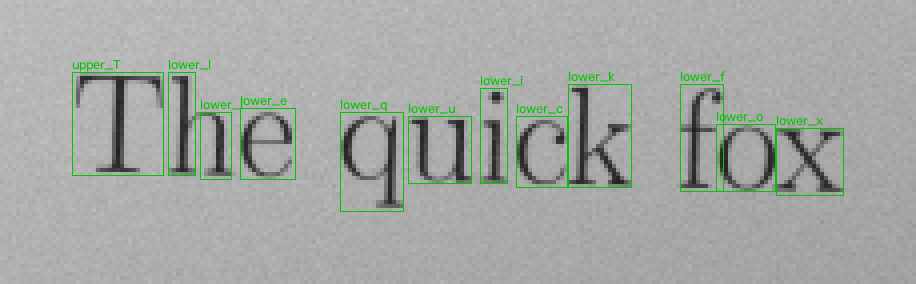
\includegraphics[width=0.86\linewidth]{img/triage_broken.png}\\[3pt]
{\small (a)}\\[5pt]
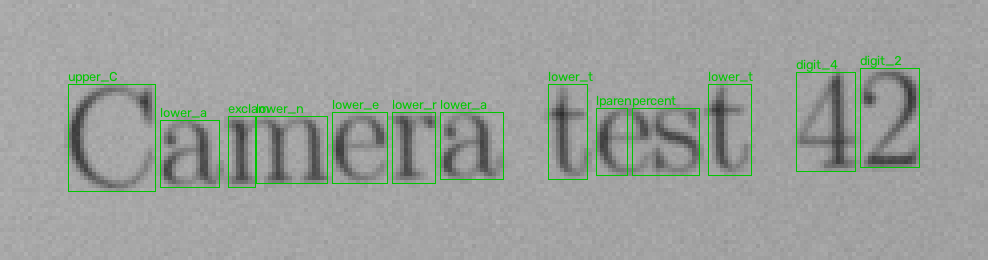
\includegraphics[width=0.92\linewidth]{img/triage_merged.png}\\[3pt]
{\small (b)}\\[5pt]
\begin{minipage}[b]{0.34\linewidth}\centering
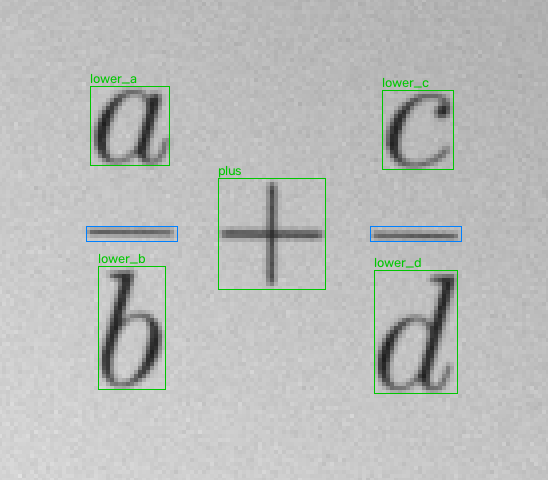
\includegraphics[height=3.6cm]{img/triage_ok.png}\\[3pt]{\small (c)}
\end{minipage}\hfill
\begin{minipage}[b]{0.38\linewidth}\centering
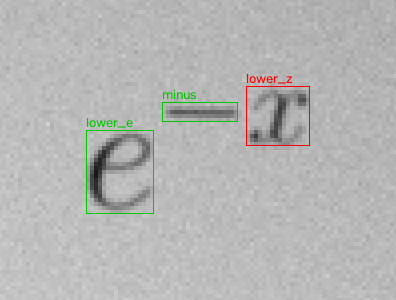
\includegraphics[height=2.6cm]{img/triage_recog.png}\\[3pt]{\small (d)}
\end{minipage}\hfill
\begin{minipage}[b]{0.24\linewidth}\centering
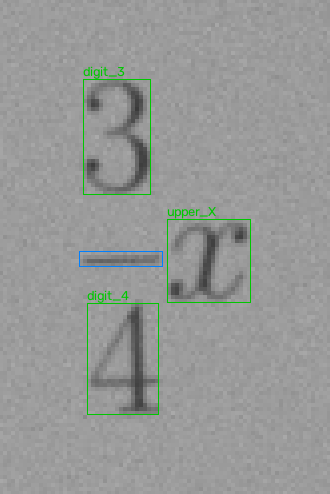
\includegraphics[height=3.6cm]{img/triage_layout.png}\\[3pt]{\small (e)}
\end{minipage}
\caption{Simulated photographs as the review document shows them, with the box and the name of
every symbol. (a)~A cutting error: the letter \emph{h} has broken into two boxes. (b)~Two
cutting errors: the \emph{m} is broken, and the letters \emph{e} and \emph{s} share boxes.
(c)~A line cut and named correctly; the bars of fractions are blue. (d)~A recognition error:
every symbol has one box, but the \emph{x} is named \emph{z}; the red box marks a symbol about
which the network was uncertain. (e)~A layout error: boxes and names are right, but the
\emph{x} was written as a superscript.}
\label{fig:triage}
\end{figure}

\begin{table}[H]
\centering
\begin{tabular}{C{1.0cm}L{2.5cm}L{7.6cm}}
\toprule
\hd{Code} & \multicolumn{1}{c}{\hd{Kind of error}} & \multicolumn{1}{c}{\hd{How it shows in the review document}} \\
\midrule
P & Photograph & The line is not wholly in the picture, a second line lies near the middle, a
  shadow or a bright spot crosses the line, or the picture is blurred by movement \\
C1 & Cutting: broken & One printed symbol has two or more boxes \\
C2 & Cutting: joined & Two or more printed symbols share one box \\
C3 & Cutting: lost or extra & A printed symbol has no box (usually a dot or a thin bar), or a box
  stands where nothing is printed \\
R & Recognition & Every symbol has exactly one box, but the name above a box is wrong \\
L & Layout & Boxes and names are right, but the \LaTeX{} is not: a wrong member of a look-alike
  group, a missing or extra space, a wrong superscript or subscript, a wrong fraction \\
\bottomrule
\end{tabular}
\caption{Kinds of error. When several apply to one line, the earliest stage counts: P before C,
C before R, R before L.}
\label{tab:kinds}
\end{table}

\subsection{The rule about the two sets of lines}

The 80 printed lines form two sets with different purposes. The 20 \term{development lines},
D01 to D20, may be examined as closely and as often as desired: every trial of this task is
judged on them. The 60 \term{test lines}, T01 to T60, measure the final accuracy and are
evaluated only at the gate of Section~\ref{sec:gate} and in Task~4. Until then, do not
evaluate them, do not open their review document, and do not choose a setting because of them.
A pipeline that has been adjusted to its own test lines reads those lines well and unknown
lines no better, and its measured accuracy would be worth nothing.

\subsection{Establish the baseline}

\step{Open the project in PowerShell}
% The opening sequence, written out in full. Input wherever a task may begin in a new window.
If a PowerShell window whose prompt begins with \texttt{(.venv)} is still open, use it and go
on to the next step. Otherwise open a new window (click \ui{Start}, type \code|powershell|,
click \ui{Windows PowerShell}) and give the two commands of the opening sequence in it.
\begin{ps}[Opening sequence, command 1 of 2]
cd C:\ee105\camera-to-latex
\end{ps}
\begin{ps}[Opening sequence, command 2 of 2]
.\.venv\Scripts\Activate.ps1
\end{ps}
\checkpoint{The prompt reads:}
\venvprompt


\step{Evaluate the development lines}\label{st:devbase}
\begin{ps}
python -m tools.eval_pipeline --split dev
\end{ps}
\begin{out}[Form of the output (the readings are the result of the measurement)]
ok D01 plain     expected Arduino Nano                 got Arduino Nano
-- D02 plain     expected Line 7: OK                   got ...
...
category   lines   exact     TER  compiles  s/line
plain         13     ...%    ...%    100.0%    ...
scripts        3     ...%    ...%    100.0%    ...
fractions      2     ...%    ...%    100.0%    ...
mixed          2     ...%    ...%    100.0%    ...
all           20     ...%    ...%    100.0%    ...

per-line results: C:\ee105\camera-to-latex\results\eval_dev_20261125_1410.csv
\end{out}
\checkpoint{The row \emph{all} reports 20 lines. If it reports fewer, photographs are missing
from \file{test\_set\bs images}: complete part~A of Task~4 first. Write down the names of the
lines that begin with \texttt{ok}; their number is the \emph{baseline}.}

\step{Produce the review document of the misread lines}\label{st:review}
Give this command directly after the evaluation, because the review program always describes
the most recent evaluation.
\begin{ps}
python -m tools.review_results --only-wrong
\end{ps}
\begin{out}
review: C:\ee105\camera-to-latex\results\review_dev_20261125_1410_wrong.pdf
\end{out}
\begin{ps}
explorer results
\end{ps}
In the Explorer window, double-click the file whose name begins with \file{review\_dev} and
ends with \file{\_wrong.pdf}. Each misread line occupies one row: at the left its photograph,
enlarged, with the boxes and names; at the right the expected line as it should be typeset, the
line as the pipeline read it (in orange), and both as \LaTeX{} text.
\checkpoint{The document shows one row for every line that the evaluation marked with
\texttt{-{}-}.}

\step{Assign every misread line to a kind of error}\label{st:triage}
For each row, compare the boxes with the printed symbols, then the names with the symbols, then
the two \LaTeX{} texts, and enter in Table~\ref{tab:triage} the first code of
Table~\ref{tab:kinds} that applies, with a few words that name the symbols concerned.

\begin{table}[H]
\centering
\begin{tabular}{C{1.3cm}C{1.3cm}L{8.2cm}}
\toprule
\hd{Line} & \hd{Code} & \multicolumn{1}{c}{\hd{What went wrong (symbols concerned)}} \\
\midrule
 & & \\[5pt] \cmidrule{1-3}
 & & \\[5pt] \cmidrule{1-3}
 & & \\[5pt] \cmidrule{1-3}
 & & \\[5pt] \cmidrule{1-3}
 & & \\[5pt] \cmidrule{1-3}
 & & \\[5pt] \cmidrule{1-3}
 & & \\[5pt] \cmidrule{1-3}
 & & \\[5pt] \cmidrule{1-3}
 & & \\[5pt] \cmidrule{1-3}
 & & \\[5pt]
\bottomrule
\end{tabular}
\caption{Triage of the misread development lines. Example of an entry: \emph{D03, C2, the
letters T and r share a box.}}
\label{tab:triage}
\end{table}
\checkpoint{Every misread line has a code. Count the lines of each code; the counts decide
which of the following subsections apply.}

\subsection{Errors of the photograph (code P)}

\step{Take the faulty photographs again}
Set up the line position as in part~A of Task~4, and give the capture command with the names of
the lines in place of the placeholder, separated by commas and without spaces:
\begin{center}
\mbox{\footnotesize\texttt{python -m pipeline.capture -{}-series test\_set\textbackslash{}images -{}-names "}\ph{NAMES}\texttt{"}}
\end{center}
\begin{out}[Example only: the command for retaking D07 and D12]
python -m pipeline.capture --series test_set\images --names "D07,D12"
\end{out}
Then repeat Steps~\ref{st:devbase} to~\ref{st:triage}. The new result is the baseline.
\checkpoint{No line carries the code P any longer.}

\subsection{Cutting errors (codes C1, C2 and C3)}
\label{sec:cutting}

Cutting errors have three possible causes, which are examined in this order: letters that are
too small or not sharp; uneven or weak light; and settings of the cutting stage that do not
suit the real photographs.

\step{Confirm the size and sharpness of the letters}
Look up the width $W$ of line T39 in the record of Task~1.
\checkpoint{$W$ lies between 280 and 300 pixels, and the trial was judged sharp. If not, the
calibration of the line position is repeated, and all 80 lines are photographed again, before
anything else is tried: no setting can restore detail that the photograph does not contain.}

\rationale{In simulated photographs read with the fallback classifier, the number of lines read
exactly rose from 57 of 80 at a capital height of 24 pixels to 63 at 28 pixels and 65 at 30
pixels, and that of the nine lines of text from one to four to six
(Table~\ref{tab:simsettings}, first row). No setting had an effect of comparable size.}

\step{Examine the light}
Open three development photographs that show cutting errors (\code|explorer test_set\images|,
then double-click) and compare the paper to the left and to the right of the line.
\checkpoint{The paper is a similar gray on both sides, the ink is clearly darker than the paper
everywhere, and no part of the line lies in a shadow. If one side is much darker, correct the
lamps as in Task~1 and take the affected photographs again.}

\subsubsection*{Trials of settings}
\label{sec:trials}

The cutting stage is governed by a few settings of \file{config.py}. Table~\ref{tab:candidates}
lists the four that are worth a trial and says which kind of error each might reduce.
Table~\ref{tab:simsettings} shows what the same settings, and some others, did in simulation.
Its message is sobering and should be kept in mind: no setting improved the reading at every
size, and several settings that look plausible did serious harm. It is therefore a legitimate
and likely outcome of this subsection that every trial is rejected and the settings remain as
they are.

\begin{table}[H]
\centering
\begin{tabular}{L{3.0cm}C{1.2cm}C{1.2cm}L{5.4cm}}
\toprule
\multicolumn{1}{c}{\hd{Setting}} & \hd{Now} & \hd{Trial} & \multicolumn{1}{c}{\hd{Intended effect}} \\
\midrule
\texttt{THRESH\_WEAK\_C} & 5 & 3 & Faint ink that touches certain ink is kept more readily;
  may mend broken strokes (C1) \\
\texttt{THRESH\_C} & 10 & 8 & A pixel needs to be less dark to count as ink; may mend broken
  strokes and lost dots (C1, C3) \\
\texttt{THRESH\_C} & 10 & 12 & A pixel must be darker to count as ink; may separate letters
  that touch, and remove boxes on bare paper (C2, C3) \\
\texttt{THRESH\_BLOCK} & 31 & 41 & The surroundings with which a pixel is compared are larger;
  may help when letters are large and their strokes thick (C1) \\
\bottomrule
\end{tabular}
\caption{Candidate settings for the trials. Each is tried alone, starting from the baseline.}
\label{tab:candidates}
\end{table}

\begin{table}[H]
\centering
\begin{tabular}{L{4.2cm}C{1.7cm}C{1.7cm}C{1.7cm}}
\toprule
\multicolumn{1}{c}{\hd{Setting changed}} & \hd{24 px} & \hd{28 px} & \hd{30 px} \\
\midrule
None (the present settings) & 57 & 63 & 65 \\
\texttt{THRESH\_WEAK\_C = 3} & 60 & 61 & 65 \\
\texttt{THRESH\_C = 8} & 56 & 62 & 64 \\
\texttt{THRESH\_C = 12} & 57 & 63 & 65 \\
\texttt{THRESH\_BLOCK = 41} & 62 & 61 & 65 \\
\midrule
\texttt{THRESH\_BLOCK = 21} & 50 & 55 & 62 \\
\texttt{THRESH\_WEAK\_C = None} & 49 & 53 & 61 \\
\texttt{CLOSE\_KSIZE = 2} & 53 & 59 & 61 \\
\texttt{BLUR\_KSIZE = 5} & 49 & 53 & 56 \\
\texttt{BLUR\_KSIZE = 0} & 16 & 15 & 16 \\
\texttt{SPACE\_GAP = 0.5} & 56 & 60 & 60 \\
\texttt{LAYOUT\_LEVEL = 2} & 44 & 50 & 52 \\
\bottomrule
\end{tabular}
\caption{Simulation: lines read exactly, of 80, at three capital heights, with one setting
changed at a time (fallback classifier, simulated photographs, 24 November). The settings
below the middle rule did harm at every size and are not to be tried.}
\label{tab:simsettings}
\end{table}

\step{Prepare two sets of simulated photographs at the calibrated size}\label{st:sims}
The simulated photographs of the quick start have capitals of 24 pixels. These two commands
produce 80 photographs each at 29 pixels, the middle of the calibrated range, with different
random tilts, lighting and noise.
\begin{ps}
python -m tools.make_test_lines --render --cap-px 29 --out data\sim0
\end{ps}
\begin{ps}
python -m tools.make_test_lines --render --cap-px 29 --seed 1 --out data\sim1
\end{ps}
\begin{out}[After the second command]
80 fake photos (29 px capitals) -> data\sim1
\end{out}
Now measure the baseline on both sets. The option \code|--no-compile| omits the check that each
reading compiles, which is not needed here and takes most of the time; the column
\emph{compiles} of the table then shows \emph{nan}. The option \code|--quiet| prints the table
alone.
\begin{ps}
python -m tools.eval_pipeline --images data\sim0 --split all --no-compile --quiet
\end{ps}
\begin{ps}
python -m tools.eval_pipeline --images data\sim1 --split all --no-compile --quiet
\end{ps}
\checkpoint{For each of the two tables, multiply the percentage in the row \emph{all} by 80 to
obtain the number of lines read exactly (78.8\,\% of 80 lines is 63 lines), and enter the sum
of the two numbers in the row \emph{baseline} of Table~\ref{tab:trialrec}.}

\step{Carry out one trial}\label{st:trial}
A trial changes a single setting and compares the result with the baseline.
\begin{enumerate}
\item Change the setting to its trial value by the method of Section~\ref{sec:setting}, and
  check that the file is valid (Step~\ref{st:valid}).
\item Evaluate the development lines:
\begin{ps}
python -m tools.eval_pipeline --split dev
\end{ps}
\item Compare the list with that of the baseline, line by line. Count the lines that are now
  \texttt{ok} and were not (\emph{gained}), and the lines that were \texttt{ok} and are no
  longer (\emph{lost}).
\item If no line was gained, or more were lost than gained, the trial has failed: go to item~6.
\item Otherwise evaluate the two simulated sets with the two commands at the end of
  Step~\ref{st:sims}, and add up the lines read exactly.
\item Enter the trial in Table~\ref{tab:trialrec}, and apply the rule below.
\end{enumerate}

\begin{plain}{The rule of adoption}
A setting is adopted only if \emph{both} conditions hold: on the 20 real development
photographs it gains at least two lines and loses none; and on the 160 simulated photographs it
reads at least as many lines as the baseline.
\end{plain}

\rationale{The pipeline contains no element of chance, so that the same photographs always give
the same reading, and a line gained on these photographs is a fact. What remains uncertain is
whether the gain will hold for other photographs. Twenty lines cannot settle that
(Section~\ref{sec:stat}); the 160 simulated photographs serve as a second, independent
witness. The rule is deliberately strict, because an adopted setting that does harm is
discovered only in the demonstration.}

\step{After a rejected trial: restore the settings}
\begin{ps}
git restore config.py
\end{ps}
\checkpoint{The command prints nothing. The file is again as it was at the last commit.}

\step{After an adopted trial: record the setting}
\begin{ps}
git add config.py
\end{ps}
\begin{ps}
git commit -m "Adopt a cutting setting after a trial on the development lines"
\end{ps}
The adopted state is now the baseline for any further trial: its list of \texttt{ok} lines and
its number of simulated lines replace the earlier ones.
\checkpoint{The second command printed a line that begins with \texttt{[main}.}

\begin{table}[H]
\centering
\begin{tabular}{L{3.4cm}C{1.45cm}C{1.1cm}C{1.95cm}C{2.6cm}}
\toprule
\multicolumn{1}{c}{\hd{Setting and value}} & \hd{Gained} & \hd{Lost} & \hd{Simulated, of 160} & \hd{Adopted?} \\
\midrule
Baseline & -- & -- & & -- \\
 & & & & \cbox\ yes\ \ \cbox\ no \\
 & & & & \cbox\ yes\ \ \cbox\ no \\
 & & & & \cbox\ yes\ \ \cbox\ no \\
 & & & & \cbox\ yes\ \ \cbox\ no \\
\bottomrule
\end{tabular}
\caption{Record of the trials. \emph{Gained} and \emph{lost} refer to the 20 development
lines.}
\label{tab:trialrec}
\end{table}

\begin{caution}[Settings that are not to be changed]
The settings below the middle rule of Table~\ref{tab:simsettings} are left alone. In
particular, \texttt{BLUR\_KSIZE = 0} looks like a way to obtain sharper letters and destroys
the reading almost completely, because the noise of the sensor then turns into ink. The
orientation settings of Task~1 and all settings of the classifier and of the layout are not
part of these trials either.
\end{caution}

\subsection{Recognition and layout errors (codes R and L)}
\label{sec:rl}

Errors of these two kinds cannot be removed by a setting. They are recorded here, so that the
project lead can decide what to do about them and so that the final report can describe them.

\step{Describe the recognition errors}
For every line with the code R, note which symbol was mistaken for which, and compare with the
list \emph{most common confusions} of Task~2 (Step~\ref{st:after}).
\checkpoint{The record states whether the confusions of whole lines are the same pairs that
dominate the confusions of single crops. If they are, a second round of sheet photographs
(Section~\ref{sec:round2}) is the remedy that needs no programming, and the lead decides
whether the time allows it. A very small symbol, such as a superscript, that is confused with a
similar one is to be expected at this resolution, and is reported as a limit of the method.}

\step{Describe the layout errors}
For every line with the code L, note the expected and the obtained \LaTeX{} text.
\checkpoint{The record lists them. Typical cases are a letter after a fraction that was taken
for a superscript, a colon read as a semicolon, and a capital letter chosen in place of the
small one of the same shape.}

\subsubsection*{Changes to the program (project lead only)}

A change to the Python code of the pipeline can do what no setting can, for example cut a wide
box at its thinnest place when the network is uncertain, or join the parts of a per cent sign.
It can also break what works. A change is therefore made on a separate \term{branch} of the
repository and joins the main line only if it passes three checks: the automatic tests, the
development lines under the rule of adoption, and the simulated photographs.
\begin{ps}[Start a branch for the change]
git switch -c fix-cutting
\end{ps}
After the change has been written:
\begin{ps}[Check 1: the automatic tests]
python -m pytest -q
\end{ps}
\begin{ps}[Check 2: the development lines]
python -m tools.eval_pipeline --split dev
\end{ps}
Check~3 consists of the two commands at the end of Step~\ref{st:sims}. If all three checks
pass, record the change on the branch, join the branch to the main line, and upload:
\begin{ps}
git commit -a -m "Improve the cutting of symbols in text lines"
\end{ps}
\begin{ps}
git switch main
\end{ps}
\begin{ps}
git merge fix-cutting
\end{ps}
\begin{ps}
git push
\end{ps}
If a check fails and cannot be repaired in the time available, the branch is simply left
behind: \cmd{git stash} sets the unfinished change aside, and \cmd{git switch main} returns to
the version that works.

\subsection{The gate: do fractions remain?}
\label{sec:gate}

The project plan contains a gate for 25 November: lines with fractions are read exactly in at
least 60\,\% of cases, or the support for fractions is withdrawn from what is handed in. The
gate is the first of the two occasions on which the test lines are evaluated.

\step{Evaluate the test lines once}\label{st:gaterun}
All trials are finished, and the settings are those that will be frozen.
\begin{ps}
python -m tools.eval_pipeline
\end{ps}
Without the option \code|--split| the command evaluates the 60 test lines.
\begin{out}[Form of the output: the table at the end]
category   lines   exact     TER  compiles  s/line
plain         25     ...%    ...%    ...%    ...
scripts       20     ...%    ...%    ...%    ...
fractions     10     ...%    ...%    ...%    ...
mixed          5     ...%    ...%    ...%    ...
all           60     ...%    ...%    ...%    ...
\end{out}
\checkpoint{The row \emph{all} reports 60 lines. Enter the five rows in the record
(Table~\ref{tab:t3record}), as counts: 80.0\,\% of 25 lines is 20 lines.}

\step{Decide}\label{st:gatedecide}
\begin{itemize}
\item \textbf{Six or more of the ten fraction lines were read exactly.} The target is met.
  Fractions remain, and the demonstration includes a fraction. Go to Section~\ref{sec:freeze}.
\item \textbf{Five or fewer were read exactly.} The target is missed. Fractions are not
  demonstrated, and the report states the result as measured. Whether the support is also
  switched off depends on the next step.
\end{itemize}
With ten lines the measurement is coarse: its standard error is 15 points
(Table~\ref{tab:stat}). The gate is nevertheless applied as it was agreed; the report gives the
count and names the uncertainty.

\step{Only if the target was missed: compare with fractions switched off}
Switching fractions off cannot help the fraction lines themselves, which are then certainly
misread. It is worth while only if the fraction logic damages \emph{other} lines, for example
by taking a minus sign for the bar of a fraction. Set \code|LAYOUT_LEVEL| to \code|2| by the
method of Section~\ref{sec:setting} and evaluate the same photographs again:
\begin{ps}
python -m tools.eval_pipeline --no-compile --quiet
\end{ps}
Compare the rows \emph{plain} and \emph{scripts} with those of Step~\ref{st:gaterun}. The
photographs are the same, so any difference is caused by the setting alone.
\begin{itemize}
\item If level~2 reads more plain and script lines in total, keep \code|LAYOUT_LEVEL = 2|:
  fractions are switched off for the hand-in, and the rows of this second evaluation are the
  ones that count.
\item Otherwise restore level~3 with the command below. Fractions stay enabled, because
  switching them off would gain nothing, but they are neither demonstrated nor claimed.
\end{itemize}
\begin{ps}[Only if level 3 is to be restored]
git restore config.py
\end{ps}
\checkpoint{The decision, and the counts of plain and script lines at both levels, are entered
in the record.}

\rationale{In simulation, switching fractions off did not help a single line of the other
categories at any size. It cost every fraction line and three others, which need the same part
of the program: the sum with its limits above and below (T45), a square root (T56) and a line
that contains a fraction (T60); see the last row of Table~\ref{tab:simsettings}. The comparison
is nevertheless made on the real photographs, because only they can show whether the fraction
logic misfires there.}

\subsection{The freeze}
\label{sec:freeze}

From the freeze onwards, neither the settings nor the program nor the classifier is changed,
except to repair a defect that would prevent the demonstration; after any such repair the final
measurement of Task~4 is repeated, and both results are reported.

\step{Check, record and mark the frozen version}\label{st:freeze}
\begin{ps}
python -m pytest -q
\end{ps}
\begin{ps}
git status --short
\end{ps}
\checkpoint{The tests pass. The second command prints nothing, or only the line
\texttt{\ M config.py}. If it lists other files, something has been left unrecorded: the
photographs of Task~4, part~A, are recorded by the last step of that part; for anything else,
ask the lead before continuing.}
If \file{config.py} is listed, record it:
\begin{ps}
git add config.py
\end{ps}
\begin{ps}
git commit -m "Settings frozen for the demonstration"
\end{ps}
Then upload the main line, and attach a \term{tag}, a permanent name for exactly this version:
\begin{ps}
git push
\end{ps}
\begin{ps}
git tag -a v1.0-rc1 -m "Frozen for the final measurement and the demonstration"
\end{ps}
\begin{ps}
git push origin v1.0-rc1
\end{ps}
\begin{ps}
git rev-parse --short HEAD
\end{ps}
\checkpoint{The last command prints seven letters and digits, the short name of the frozen
commit. Enter it in the record. The tag is visible on the GitHub page of the repository under
\emph{Tags}.}

\step{Fill in the record}
\begin{table}[H]
\centering
\begin{tabular}{L{7.2cm}C{4.0cm}}
\toprule
\multicolumn{1}{c}{\hd{Quantity}} & \hd{Value} \\
\midrule
Development lines read exactly at the baseline (of 20) & \\
Misread lines by kind: P; C1; C2; C3; R; L & \\
Settings adopted (name and value), or \emph{none} & \\
Development lines read exactly at the freeze (of 20) & \\
Simulated lines read exactly at the freeze (of 160) & \\
Gate, plain lines read exactly (of 25) & \\
Gate, script lines (of 20) & \\
Gate, fraction lines (of 10) & \\
Gate, mixed lines (of 5) & \\
Gate, all lines (of 60) & \\
Plain and script lines at level 2, if compared (of 45) & \\
\texttt{LAYOUT\_LEVEL} at the freeze; fractions demonstrated? & \\
Short name of the frozen commit; date & \\
\bottomrule
\end{tabular}
\caption{Record of Task 3.}
\label{tab:t3record}
\end{table}

\section{Task 4: The test lines and the accuracy on real photographs}
\sectionmark{Task 4: Test lines and accuracy}
\label{sec:t4}

\subsection{Purpose, conditions and criterion}

\begin{plain}{Task 4 at a glance}
\textbf{Purpose.} The accuracy figures known so far come from simulated photographs. This task
replaces them by measurements on real ones. In part~A the 80 printed lines are photographed
with the board. In part~B, after the pipeline has been frozen, the 60 test lines among them are
evaluated once, and the result is compared with the targets of the project.

\textbf{Before you begin.} For part~A: Task~1 is complete, the line platform exists, and the 16
printed pages of test lines are at hand. For part~B: Task~3 is complete, and the frozen version
carries the tag \texttt{v1.0-rc1}.

\textbf{Complete when.} Part~A: 80 photographs exist, each shows the whole of the line after
which it is named, and they are stored in the repository. Part~B: the table of results against
targets (Table~\ref{tab:targets}) is filled in with counts, and the per-line results and the
review document are stored in the team's shared folder.

\textbf{Time.} Part~A about one hour; part~B about half an hour.
\end{plain}

\subsection{Part A: photograph the 80 lines}
\label{sec:t4a}

Part~A may be carried out while the classifier of Task~2 trains. In that case it needs a second
PowerShell window, and the window in which the training runs must be left alone.

\step{Open a PowerShell window for the photography}
Click \ui{Start}, type \code|powershell|, and click \ui{Windows PowerShell}. A new window opens.
In it, give the two commands of the opening sequence:
\begin{ps}[Opening sequence, command 1 of 2]
cd C:\ee105\camera-to-latex
\end{ps}
\begin{ps}[Opening sequence, command 2 of 2]
.\.venv\Scripts\Activate.ps1
\end{ps}
\checkpoint{The prompt of the new window reads:}
\venvprompt

\step{Set up the line position}
Put the line platform back on its outline, with a blank white sheet on top, and check the lamps
as in Task~1. Sort the 16 printed pages by the names at their right margins: the pages with T01
to T60 first, then those with D01 to D20.
\checkpoint{The platform has the thickness entered in the record of Task~1, and the pages are
in order.}

\step{Start the series}\label{st:lineseries}
\begin{pswide}
python -m pipeline.capture --series test_set\images --names-file test_set\photo_names.txt
\end{pswide}
The viewfinder opens, and its yellow line reads \emph{1/80\ \ next: T01}. The names follow the
order of the printed pages.
\checkpoint{The viewfinder shows the live picture and the name \emph{T01}.}

\step{Photograph each line}\label{st:oneline}
For each of the 80 lines:
\begin{enumerate}
\item Lay the page on the platform, its top towards the arrow, and move it until the line named
  in the viewfinder lies in the middle of the picture. The name is printed at the right margin
  of the page, level with the line, and is itself outside the picture.
\item Check four things in the viewfinder. The whole line is inside the picture, with white
  paper beyond its first and its last symbol. The line lies in the middle third of the height
  of the picture and runs parallel to the border, its two ends at the same height to within
  half a letter. No shadow and no bright spot touches it. For a fraction or a sum, the whole
  structure is inside, top to bottom.
\item Wait until the picture has stood still for two seconds, and press \key{Space}.
\end{enumerate}
Parts of the neighbouring lines appear at the upper and lower borders of the picture. They are
left as they are: the program reads the row nearest the middle, and covering the neighbours
would only add the edges and shadows of the covering sheets. Line T39 is the only one that
nearly fills the width of the picture; centre it with particular care.
\checkpoint{After the 80th photograph the viewfinder closes by itself.}

\begin{note}[Mistakes and interruptions]
As in Task~2: \key{B} goes back one name so that a photograph can be replaced; \key{Q}
interrupts the series; when the command is given again, \key{N} passes over the names marked
\emph{(exists)}. Single photographs are taken again with the placeholder form of the command,
in which the names are separated by commas and enclosed in quotation marks:
\begin{center}
\mbox{\footnotesize\texttt{python -m pipeline.capture -{}-series test\_set\textbackslash{}images -{}-names "}\ph{NAMES}\texttt{"}}
\end{center}
For example, \code|--names "T17,T23"| at the end of the command retakes the lines T17 and T23.
\end{note}

\step{Count and inspect the photographs}
\begin{ps}
(Get-ChildItem test_set\images -Filter *.png).Count
\end{ps}
\checkpoint{The answer is \texttt{80}.}
\begin{ps}
explorer test_set\images
\end{ps}
In the Explorer window choose \menu{View}\then\menu{Extra large icons} and look at all 80
photographs. Each must show one whole line in the middle of the picture, upright and sharp.
Then compare five photographs with the printed lines of the same names: T05, T25, T45, T60 and
D20.
\checkpoint{Every photograph shows a whole line, and the five photographs show the lines after
which they are named. A photograph that shows the neighbour of its line means that a line was
skipped or taken twice; from that point on the names are shifted, and the affected photographs
are taken again.}

\step{Let the pipeline read the development lines}
The 20 development lines, and only they, may be evaluated at once; the test lines wait for
part~B.
\begin{ps}
python -m tools.eval_pipeline --split dev --no-compile --quiet
\end{ps}
\checkpoint{The table reports 20 lines in its row \emph{all}, and a share of exact readings
that is clearly above zero. (The column \emph{compiles} shows \emph{nan}, because that check
was omitted.) A share of zero means that the photographs are unusable as a set:
the names are shifted, or the orientation setting of Task~1 is missing on this laptop.}

\step{Store the photographs in the repository}
\begin{ps}
git add test_set\images
\end{ps}
\begin{ps}
git commit -m "Photographs of the 80 test and development lines"
\end{ps}
\begin{ps}
git push
\end{ps}
\checkpoint{The output of the last command ends with a line that contains \texttt{main ->
main}.}

\step{Fill in the record of part A}
\begin{table}[H]
\centering
\begin{tabular}{L{7.4cm}C{3.8cm}}
\toprule
\multicolumn{1}{c}{\hd{Quantity}} & \hd{Value} \\
\midrule
Date; photographer & \\
Thickness of the platform; width $W$ of T39 in \file{T39.png} & \\
Lamps (number, position) & \\
Photographs taken; photographs retaken & \\
Print size of the lines & \\
\bottomrule
\end{tabular}
\caption{Record of Task 4, part A. The width of T39 is measured in Paint as in Task~1, with
the command \texttt{mspaint test\_set\bs images\bs T39.png}.}
\label{tab:t4arecord}
\end{table}

\subsection{Part B: the final measurement}
\label{sec:t4b}

The final measurement is made once, on the frozen version. Its result is reported whatever it
is; a target that is missed is reported as missed.

\step{Open the project in PowerShell}
% The opening sequence, written out in full. Input wherever a task may begin in a new window.
If a PowerShell window whose prompt begins with \texttt{(.venv)} is still open, use it and go
on to the next step. Otherwise open a new window (click \ui{Start}, type \code|powershell|,
click \ui{Windows PowerShell}) and give the two commands of the opening sequence in it.
\begin{ps}[Opening sequence, command 1 of 2]
cd C:\ee105\camera-to-latex
\end{ps}
\begin{ps}[Opening sequence, command 2 of 2]
.\.venv\Scripts\Activate.ps1
\end{ps}
\checkpoint{The prompt reads:}
\venvprompt


\step{Confirm that the frozen version is in use}
\begin{ps}
git pull
\end{ps}
\begin{ps}
git status --short
\end{ps}
\begin{ps}
git describe --tags
\end{ps}
\checkpoint{The second command prints nothing: no file differs from the repository. The third
prints \texttt{v1.0-rc1}. If it prints a longer name, such as \texttt{v1.0-rc1-2-g3f2c1ab},
commits have been added since the freeze; ask the lead whether they were intended.}

\step{Evaluate the 60 test lines}\label{st:final}
\begin{ps}
python -m tools.eval_pipeline
\end{ps}
The command reads the 60 photographs T01 to T60, compares each reading with the expected
\LaTeX{}, checks that each reading compiles, prints one line for each photograph and the table
of Step~\ref{st:gaterun}, and names the file in which the per-line results are stored.
\checkpoint{The row \emph{all} reports 60 lines. The table is identical to that of the gate of
Task~3, because neither the photographs nor the pipeline have changed and the pipeline contains
no element of chance. A difference means that something has changed since the gate; find out
what before any figure is reported.}

\step{Produce the review document}
\begin{ps}
python -m tools.review_results
\end{ps}
\begin{out}
review: C:\ee105\camera-to-latex\results\review_test_20261130_1012.pdf
\end{out}
\checkpoint{The file exists. It shows all 60 lines, each with its photograph, the boxes, the
expected line and the reading; misread lines are marked in orange.}

\step{Compare the result with the targets}
Convert each percentage of the table into a count, and fill in Table~\ref{tab:targets}. The
accuracy on single symbols comes from the record of Task~2, and the time per picture from the
soak test of Task~1.

\begin{table}[H]
\centering
\begin{tabular}{L{4.5cm}C{2.5cm}C{2.0cm}C{1.5cm}}
\toprule
\multicolumn{1}{c}{\hd{Quantity}} & \hd{Target} & \hd{Result} & \hd{Met?} \\
\midrule
Symbols named correctly (held-out real crops) & 95 \% & \hfill of 280 & \\
Plain lines read exactly & 80 \% (20 of 25) & \hfill of 25 & \\
Script lines read exactly & 70 \% (14 of 20) & \hfill of 20 & \\
Fraction lines read exactly & 60 \% (6 of 10) & \hfill of 10 & \\
Mixed lines read exactly & no target & \hfill of 5 & -- \\
All test lines read exactly & no target & \hfill of 60 & -- \\
Readings that compile & 100 \% & \hfill of 60 & \\
Time from key press to reading & 5 s or less & \hfill s & \\
\bottomrule
\end{tabular}
\caption{Results against the targets of the project plan. The time from key press to reading is
the time per picture of the soak test plus the value in the column \emph{s/line} of the
evaluation. In the application a line can be accepted only if it compiles, so that every
accepted line compiles by construction; the row on compiling reports how many readings
compiled exactly as they were produced.}
\label{tab:targets}
\end{table}
\checkpoint{Every row has a result. Each result is a count, so that its precision can be
judged (Section~\ref{sec:stat}).}

\step{Classify the misread lines}
Open the review document (\code|explorer results|, then double-click the file whose name begins
with \file{review\_test}) and assign every misread line to a kind of error by
Table~\ref{tab:kinds}, as in Step~\ref{st:triage}. Mark three or four lines that show different
kinds of error clearly; the final report presents them as examples.
\checkpoint{The record states how many misread lines fall under each code. This analysis
serves the report alone: nothing in the pipeline is changed because of it.}

\step{Store the evidence}
In the Explorer window of the folder \file{results}, sort by date. Upload the two newest files
whose names begin with \file{eval\_test} and \file{review\_test} to the team's shared Google
Drive folder (\menu{New}\then\menu{File upload}).
\checkpoint{Both files are visible in the shared folder. The final report takes its figures and
its examples from them.}

\step{Enter the result in the table of the README (project lead)}
The file \file{README.md} of the repository contains a table headed \emph{Results}, with one
row for each measurement.
\begin{ps}
notepad README.md
\end{ps}
Press \key{Ctrl}+\key{F}, type \code|## Results| and press \key{Enter}; Notepad jumps to the
heading of the table. Select the last row of the table, which is one long line that begins and
ends with a vertical bar, copy it, and paste the copy on a new line below it. In the copy,
replace the entries between the bars by today's date, the version \code|v1.0-rc1|, the words
\emph{60 real test lines}, the capital height of Task~1, the classifier, and the counts of
Table~\ref{tab:targets}. Keep every vertical bar. Save with \key{Ctrl}+\key{S}, close Notepad,
and record the change:
\begin{ps}
git add README.md
\end{ps}
\begin{ps}
git commit -m "Results of the final measurement on real photographs"
\end{ps}
\begin{ps}
git push
\end{ps}
\checkpoint{On the GitHub page of the repository, the table shows the new row.}

\step{Fill in the record of part B}
\begin{table}[H]
\centering
\begin{tabular}{L{7.4cm}C{3.8cm}}
\toprule
\multicolumn{1}{c}{\hd{Quantity}} & \hd{Value} \\
\midrule
Date; version (output of \texttt{git describe -{}-tags}) & \\
Name of the per-line results file & \\
Table identical to that of the gate? & \cbox\ yes\quad\cbox\ no \\
Misread test lines by kind: P; C1; C2; C3; R; L & \\
Lines chosen as examples for the report & \\
\bottomrule
\end{tabular}
\caption{Record of Task 4, part B. The results themselves are in Table~\ref{tab:targets}.}
\label{tab:t4brecord}
\end{table}

\section{Task 5: The demonstration video}
\sectionmark{Task 5: Demonstration video}
\label{sec:t5}

\subsection{Purpose, conditions and criterion}

\begin{plain}{Task 5 at a glance}
\textbf{Purpose.} A video of one minute or less shows the complete system at work: a printed
line is laid below the camera, a key is pressed, the line appears as \LaTeX{}, and after three
lines the typeset PDF opens. The video is handed in through Google Drive, and it is also the
last line of defence of the live demonstration, should the hardware fail on the day.

\textbf{Before you begin.} Task~3 is complete (the pipeline is frozen), and the list of test
lines that were read correctly is available from part~B of Task~4. The recording takes place at
the stand of Task~1. The simplest arrangement is to use the laptop on which Tasks~1 to~4 were
carried out. Any other laptop must have completed the Set-up Guide, except that the two long
steps that generate training images and train the classifier are replaced by \cmd{git pull},
which fetches the team's classifier; and Step~\ref{st:ping} of this document must succeed on
it. A telephone with a camera is needed, and something to hold it still.

\textbf{Complete when.} (1)~The video lasts 60 seconds or less and shows three lines being read
and the resulting PDF. (2)~It is in Google Drive, and its link opens in a browser window that is
not signed in. (3)~The link is entered in the report and has been sent to the team. (4)~A copy
of the file is on the laptop that will be used for the live demonstration.

\textbf{Time.} About an hour and a half, most of it rehearsal.
\end{plain}

\subsection{Choose the three lines}

\step{Select candidates from the results}
The video shows one line of each kind: ordinary text, a formula with superscripts, and a
fraction. If the gate of Task~3 decided that fractions are not demonstrated, the third line is
a second formula. Choose only lines that the frozen pipeline read correctly, that is, lines
marked \texttt{ok} in the final measurement (Step~\ref{st:final}). Table~\ref{tab:cards} lists
suitable lines.

\begin{table}[H]
\centering
\begin{tabular}{C{2.3cm}C{1.3cm}C{3.3cm}C{1.3cm}C{2.0cm}}
\toprule
\hd{Kind} & \hd{Line} & \hd{Content} & \hd{Page} & \hd{Mode} \\
\midrule
Text & T01 & Hello World & 1 & text \\
Text & T03 & ECE 105 Lab & 1 & text \\
Superscripts & T26 & $x^{2}+y^{2}=r^{2}$ & 6 & math \\
Superscripts & T27 & $E=mc^{2}$ & 6 & math \\
Fraction & T54 & $\dfrac{a+b}{2}$ & 11 & math \\[7pt]
Fraction & T47 & $\dfrac{a}{b}+\dfrac{c}{d}$ & 10 & math \\[7pt]
Fraction & T46 & $\dfrac{1}{2}$ & 10 & math \\[5pt]
\bottomrule
\end{tabular}
\caption{Lines suitable for the video and for the live demonstration. The pages are those of
the test lines printed at 40\,pt.}
\label{tab:cards}
\end{table}
\checkpoint{Three lines are chosen, one of each kind, all of them marked \texttt{ok} in the
final measurement. Their pages, printed a second time, are the \emph{cards} of the
demonstration.}

\step{Open the project in PowerShell}
% The opening sequence, written out in full. Input wherever a task may begin in a new window.
If a PowerShell window whose prompt begins with \texttt{(.venv)} is still open, use it and go
on to the next step. Otherwise open a new window (click \ui{Start}, type \code|powershell|,
click \ui{Windows PowerShell}) and give the two commands of the opening sequence in it.
\begin{ps}[Opening sequence, command 1 of 2]
cd C:\ee105\camera-to-latex
\end{ps}
\begin{ps}[Opening sequence, command 2 of 2]
.\.venv\Scripts\Activate.ps1
\end{ps}
\checkpoint{The prompt reads:}
\venvprompt


\step{Confirm each line at the stand}\label{st:confirm}
A line that was read correctly once in a stored photograph may still fail under slightly
different light. Set up the line position, start the application,
\begin{ps}
python -m pipeline.main --new
\end{ps}
and read each of the three lines five times, moving the page a little between readings: press
\key{Space}, compare the reading below the picture with the printed line, and press \key{R}.
Before the text line, press \key{M} until the status line below the picture says \emph{mode
text}; before the formulas, until it says \emph{mode math}. Finish with \key{Q}.
\checkpoint{Each of the three lines was read exactly right at least four times out of five. A
line that fails more often is replaced by another line of Table~\ref{tab:cards} and confirmed
in the same way.}

\subsection{Prepare the scene}

\step{Arrange the screen}
The viewer must be able to read the screen in the video. Three windows matter: the application
window with the picture of the camera, the PowerShell window in which the readings are printed,
and the PDF that opens at the end.
\begin{enumerate}
\item Enlarge everything on the screen: open \menu{Settings}\then\menu{System}\then\menu{Display}
  and, under \ui{Scale}, choose the next larger value, for example 150\,\% in place of
  125\,\%. Note the previous value, so that it can be restored afterwards.
\item Start the application (the command of Step~\ref{st:confirm}). Drag the application window
  to the left half of the screen and the PowerShell window to the right half.
\item Close every window that shows an earlier \file{document.pdf}. Some PDF readers lock the
  file while it is open, and the application could then not write the new one.
\end{enumerate}
\checkpoint{Both windows are visible side by side, and no PDF is open.}

\step{Arrange the camera of the telephone}
Hold the telephone horizontally and fix it, on a tripod or leaning against a stack of books,
about 70\,cm from the desk, so that its picture contains both the stand, with the page below
the board, and the laptop screen. Switch off the flash. Record a test of ten seconds and look
at it.
\checkpoint{In the test recording the page below the board can be seen, the text below the
picture in the application window can be read, and no lamp is reflected in the laptop screen.}

\subsection{Rehearse and record}

\step{Learn the sequence}
Table~\ref{tab:storyboard} gives the sequence of the video with the time that each part may
take. The keys act on the application window, which must be the active window: click on its
picture once before starting.

\begin{table}[H]
\centering
\begin{tabular}{C{1.6cm}L{5.0cm}L{4.3cm}}
\toprule
\hd{Seconds} & \multicolumn{1}{c}{\hd{Action}} & \multicolumn{1}{c}{\hd{Words (optional)}} \\
\midrule
0--6 & Show the stand; point to the board & ``An EE\,105 board photographs one printed line.'' \\
6--20 & Press \key{M} until \emph{mode text}. Lay the first card; wait for the picture; press
  \key{Space}, then \key{A} & ``The laptop cuts the photograph into symbols and names each one.'' \\
20--33 & Press \key{M} for \emph{mode math}. Lay the second card; \key{Space}, then \key{A} &
  ``Positions and sizes give the superscripts.'' \\
33--46 & Lay the third card; \key{Space}, then \key{A} & ``A bar with symbols above and below
  becomes a fraction.'' \\
46--58 & Press \key{P}; the PDF opens & ``The accepted lines are typeset by \LaTeX{} into a PDF.'' \\
\bottomrule
\end{tabular}
\caption{Sequence of the video. After the space bar, wait until the boxes and the reading have
appeared before pressing the key A; after the key A, wait until the live picture has returned.}
\label{tab:storyboard}
\end{table}

What each key does is shown in the PowerShell window: after \key{Space} the reading is printed;
after \key{A} the line \emph{accepted line 1}, followed by the reading; after \key{P} the path
of the PDF, which then opens in the PDF reader of the laptop.

\step{Rehearse with a stopwatch}
Run through the whole sequence three times without recording, with the stopwatch of the
telephone. Begin each run with a fresh session: press \key{Q} in the application window, close
the PDF, and start the application again with the command of Step~\ref{st:confirm}.
\checkpoint{One complete run took 58 seconds or less, and all three readings were correct. If
the runs are too long, omit the spoken words and the first six seconds; if they are still too
long, show two lines.}

\step{Record}
Start a fresh session as before, start the recording on the telephone, and carry out the
sequence. If a reading is wrong, stop and begin again; a video of the demonstration should not
need an excuse. Record until two takes are free of errors, and keep the better one.
\checkpoint{The chosen take lasts 60 seconds or less from its first to its last picture, all
three readings in it are correct, and the PDF at the end shows the three lines. If the take
has a few idle seconds at its beginning or end, trim them with the editing function of the
telephone's photo application; do not cut anything out of the middle.}

\step{Restore the screen}
Set \ui{Scale} back to its previous value (\menu{Settings}\then\menu{System}\then\menu{Display}).

\subsection{Upload and share}

\step{Upload the video to Google Drive}
On the telephone, open the Google Drive application, signed in with the USC account. Tap the
\ui{+} button, then \ui{Upload}, and select the video. Give the upload time to finish on a
wireless network.
\checkpoint{The video appears in \emph{My Drive} and plays when it is tapped.}

\step{Allow others to view it}\label{st:share}
On the laptop, open \url{https://drive.google.com} in the browser, signed in with the same
account. Right-click the video and choose \menu{Share}\then\menu{Share}. Under \ui{General
access}, change \ui{Restricted} to \ui{Anyone with the link}, and leave the role at
\ui{Viewer}. Click \ui{Copy link}, then \ui{Done}.
\checkpoint{The link is in the clipboard.}

\begin{iffail}[If ``Anyone with the link'' is not offered]
The university may restrict sharing. Choose the entry with the name of the university in its
place; every member of the university who is signed in can then view the video. Ask a teammate
to open the link as a check.
\end{iffail}

\step{Verify the link as a stranger would see it}
Open a private window of the browser (\key{Ctrl}+\key{Shift}+\key{N} in Chrome and Edge), paste
the link into the address bar with \key{Ctrl}+\key{V}, and press \key{Enter}.
\checkpoint{The video plays in the private window without any request to sign in. Its length,
shown at the right of the player's time bar, is 1:00 or less.}

\step{Deliver the link and keep a copy}
Paste the link into the place where the course's report template asks for videos, and send it
to the team. Download the video to the laptop that will be used for the live demonstration
(right-click the video in Google Drive, then \menu{Download}), and check that the downloaded
file plays without a network connection.
\checkpoint{The report contains the link, and the file plays on the demonstration laptop with
the wireless network switched off.}

\subsection{If the board is not available}
\label{sec:noboard}

Should the board be unavailable when the video must be recorded, the pipeline can be shown on
the stored photographs of the same three lines. This is a substitute, and the video must say
so: the spoken words, or a caption, state that stored photographs taken earlier with the board
are being read. The three commands below read the photographs of the default lines T01, T26 and
T54; each shows its result in a window until a key is pressed, and the last one builds and
opens the PDF. Each command needs some seconds to start.
\begin{pswide}[Stored photograph of the text line]
python -m pipeline.main --new --mode text --image test_set\images\T01.png --show --accept
\end{pswide}
\begin{ps}[Stored photograph of the line with superscripts]
python -m pipeline.main --mode math --image test_set\images\T26.png --show --accept
\end{ps}
\begin{pswide}[Stored photograph of the fraction, then the PDF]
python -m pipeline.main --mode math --image test_set\images\T54.png --show --accept --pdf
\end{pswide}
\checkpoint{After the third command, the PDF opens with three lines. The same three commands
are the first fallback of the live demonstration (Section~\ref{sec:rehearsal}).}

\subsection{Record}

\begin{table}[H]
\centering
\begin{tabular}{L{6.4cm}C{4.8cm}}
\toprule
\multicolumn{1}{c}{\hd{Quantity}} & \hd{Value} \\
\midrule
Date; persons recording and operating & \\
The three lines shown & \\
Readings correct in the confirmation (of 5, each line) & \\
Length of the video & \hfill s \\
Link checked in a private window & \cbox\ yes\quad\cbox\ no \\
Link entered in the report; copy on the demonstration laptop & \cbox\ yes\quad\cbox\ no \\
\bottomrule
\end{tabular}
\caption{Record of Task 5.}
\label{tab:t5record}
\end{table}

\section{Task 6: The final report, the presentation and the rehearsal}
\sectionmark{Task 6: Report, presentation, rehearsal}
\label{sec:t6}

\subsection{Purpose, conditions and criterion}

\begin{plain}{Task 6 at a glance}
\textbf{Purpose.} The project is judged by what is handed in on 1 December: a report, a
presentation with a live demonstration, and the repository. This task assembles them from the
records of Tasks~1 to~5, rehearses the demonstration twice on 30 November, and marks the
version that is handed in.

\textbf{Before you begin.} The official requirements of the course for the report and the
presentation are at hand (Step~\ref{st:reqs}); this section cannot replace them, and where they
differ from it, they prevail. For the sections on results: part~B of Task~4 is complete. For
the rehearsal: Tasks~1 to~5 are complete.

\textbf{Complete when.} (1)~The report contains every item that the course requires, and every
figure in it can be traced to a record of this document. (2)~The presentation has been timed
within its limit. (3)~The demonstration has been rehearsed twice, each fallback has been
practised once, and the times are recorded. (4)~The repository carries the tag \texttt{v1.0}. (5)~Everything has
been submitted where the course requires it, and the board has been returned.

\textbf{Time.} Writing as required; each rehearsal about half an hour.
\end{plain}

\subsection{Establish the requirements}

\step{Obtain the official requirements and fill in the checklist}\label{st:reqs}
Collect the course's instructions for the final report and the final presentation from the
course site, the syllabus and the instructor's announcements, and enter them in
Table~\ref{tab:reqs}. Where an item cannot be found, ask the teaching staff now and not on the
last day.

\begin{table}[H]
\centering
\begin{tabular}{L{6.0cm}L{5.2cm}}
\toprule
\multicolumn{1}{c}{\hd{Question}} & \multicolumn{1}{c}{\hd{Answer of the course}} \\
\midrule
Report: template to be used; file format & \\
Report: required sections; limit of pages or words & \\
Report: statement of each member's contribution? & \\
Report: where and by what time it is submitted & \\
Presentation: length; number of speakers & \\
Presentation: slides required? format; where submitted & \\
Demonstration: room, time, table, power sockets & \\
Demonstration: is a projector or a second screen provided? & \\
Video: where the link is entered & \\
Repository: must the staff have access? how? & \\
Board: when and where it is returned & \\
\bottomrule
\end{tabular}
\caption{The requirements of the course, to be filled in before writing begins.}
\label{tab:reqs}
\end{table}
\checkpoint{Every row has an answer, or the name of the person who has been asked.}

\subsection{Collect the evidence}

A report of measurements is only as good as its sources. Before any text is written, the
material of Table~\ref{tab:evidence} is brought together in one shared folder.

\begin{table}[H]
\centering
\begin{tabular}{L{4.6cm}L{6.6cm}}
\toprule
\multicolumn{1}{c}{\hd{Material}} & \multicolumn{1}{c}{\hd{Where it comes from}} \\
\midrule
Geometry of the stand, scale, capital height & Record of Task~1 (Table~\ref{tab:t1record}) \\
Photograph of the stand & Task~1, taken with a telephone \\
A photograph as the board delivers it & Any file of \file{test\_set\bs images}, for example
  \file{T26.png} \\
A sheet photograph with its grid & Any file of \file{data\bs sheets\bs debug} \\
Number of photographs and crops; accuracy on real crops before and after retraining; most
  common confusions & Record of Task~2 (Table~\ref{tab:t2record}) \\
Accuracy for each class & The file \file{results\bs crops\_symbols\_v1.csv}, which opens in
  Excel \\
Size and training of the network & The end of the file \file{models\bs symbols\_v1.json}
  (open it with Notepad) \\
Kinds of error; trials of settings; decision of the gate & Record of Task~3
  (Tables~\ref{tab:triage}, \ref{tab:trialrec} and~\ref{tab:t3record}) \\
Final results against the targets & Table~\ref{tab:targets} \\
Misread lines as examples & The review document of Task~4, part~B \\
A PDF produced by the system & The file \file{out\bs document.pdf} after the recording of
  the video \\
The video & The link of Task~5 \\
The version handed in & The tag of Step~\ref{st:release} \\
\bottomrule
\end{tabular}
\caption{The evidence on which the report rests.}
\label{tab:evidence}
\end{table}

\step{Open the project in PowerShell}
% The opening sequence, written out in full. Input wherever a task may begin in a new window.
If a PowerShell window whose prompt begins with \texttt{(.venv)} is still open, use it and go
on to the next step. Otherwise open a new window (click \ui{Start}, type \code|powershell|,
click \ui{Windows PowerShell}) and give the two commands of the opening sequence in it.
\begin{ps}[Opening sequence, command 1 of 2]
cd C:\ee105\camera-to-latex
\end{ps}
\begin{ps}[Opening sequence, command 2 of 2]
.\.venv\Scripts\Activate.ps1
\end{ps}
\checkpoint{The prompt reads:}
\venvprompt


\step{Copy the sample output into the repository}
The PDF that the system produced during the recording of the video is the most direct proof
that it works. Copy it into the folder of documents and record it:
\begin{ps}
Copy-Item out\document.pdf docs\sample_output.pdf
\end{ps}
\begin{ps}
git add docs\sample_output.pdf
\end{ps}
\begin{ps}
git commit -m "Sample output produced from photographs"
\end{ps}
\begin{ps}
git push
\end{ps}
\checkpoint{The file \file{sample\_output.pdf} is visible in the folder \file{docs} on the
GitHub page of the repository.}

\subsection{Write the report}

If the course provides a template, its sections are used. Table~\ref{tab:outline} lists what a
complete account of this project contains; each item belongs somewhere in the template. It
follows the outline of the project plan.

\begin{longtable}{C{0.6cm}L{3.0cm}L{7.3cm}}
\toprule
 & \multicolumn{1}{c}{\hd{Part}} & \multicolumn{1}{c}{\hd{What it must say}} \\
\midrule
\endhead
\bottomrule
\endfoot
\bottomrule
\caption{Contents of a complete report.}\label{tab:outline}\\
\endlastfoot
1 & Problem and scope & What the system does (one printed line per photograph, read into
  \LaTeX{} and collected into a PDF) and what it does not do (handwriting, several lines at
  once, recognition on the board itself) \\
2 & Hardware and its limits & The board and the camera; 256\,KB of memory, hence photographs of
  $320 \times 240$ gray pixels; the stand; the measured scale and the size of the letters \\
3 & Architecture & The stages from capture to PDF, with the diagram of the pipeline; why
  recognition runs on the laptop \\
4 & Data & The synthetic images; the 54 sheet photographs and their crops; the 60 test and 20
  development lines, and the rule that kept them apart \\
5 & Classifier & The network (159 classes for 182 symbols, 149{,}311 weights); its accuracy on
  held-out real crops before and after retraining, as counts; the common confusions \\
6 & Cutting and layout & How ink is separated from paper and formed into symbols; how
  superscripts, subscripts and fractions follow from positions and sizes \\
7 & Results & Table~\ref{tab:targets}: every target, the result as a count, whether it was
  met, and the precision of the figure \\
8 & Failures & Three or four misread lines, each with its photograph, the kind of error and the
  reason \\
9 & Limits and next steps & What a second version would change, for example recognition on the
  board, or a model that reads a whole line \\
10 & Contributions & Who did what, in the form that the course requires \\
11 & Sources & The software libraries and fonts used, and any assistance, including that of AI
  tools, in the form that the course requires \\
\end{longtable}

\step{Write the parts that do not depend on the final results}
Parts 1 to 4, 6 and 9 to 11 can be written before part~B of Task~4 is finished.
\checkpoint{These parts exist in draft, and every number in them is taken from a record or
from the repository, not from memory.}

\step{Write the results as they were measured}
Parts 5, 7 and 8 are written from Table~\ref{tab:targets} and the review document. Four rules
keep them honest and useful.
\begin{enumerate}
\item A result is given as a count and a percentage, for example ``17 of 25 lines (68\,\%)'',
  and a target that was missed is called missed.
\item Simulated and real photographs are never mixed in one figure, and each figure says which
  it is. The results of 23 November were obtained on simulated photographs.
\item The uncertainty is named where a conclusion depends on it; the formula and the values
  are in Section~\ref{sec:stat}.
\item The conditions are stated: print of 40\,pt (or 48\,pt, if the larger print was used), the
  measured distance and scale, the lighting, and the fact that each line was read in the mode,
  text or mathematics, that the operator would choose.
\end{enumerate}
\checkpoint{Every figure of the results can be found in Table~\ref{tab:targets} or in a record
of this document.}

\step{Check the report against the requirements}
Read the finished report beside Table~\ref{tab:reqs} and Table~\ref{tab:outline}.
\checkpoint{Every required section is present, the limit of length is kept, the link of the
video opens in a private browser window, and a member who did not write the report has read it
from beginning to end.}

\subsection{Prepare the presentation}

\step{Bring the slides up to date}
The team has a deck of slides from the design presentation, \emph{Camera to \LaTeX{}: how it
works and why}; the project lead shares it. Its account of the method remains valid. Three
things change for the final presentation: figures from simulation are replaced by the measured
ones; the stand and the results are shown; and time is reserved for the demonstration.
Table~\ref{tab:slides} proposes a sequence, to be shortened to the length that the course
allows.

\begin{table}[H]
\centering
\begin{tabular}{C{1.1cm}L{4.2cm}L{5.7cm}}
\toprule
\hd{Slide} & \multicolumn{1}{c}{\hd{Subject}} & \multicolumn{1}{c}{\hd{Content}} \\
\midrule
1 & Title & Project, team, date \\
2 & The task and the limits & One sentence on the aim; the three limits that shaped the design:
  memory, resolution, one line per photograph \\
3 & How it works & The diagram of the pipeline \\
4 & Data and classifier & Synthetic images and sheet photographs; accuracy on real crops,
  before and after \\
5 & The stand & Its photograph; distance, scale, size of the letters \\
6 & Results & Table~\ref{tab:targets}, as counts, with the targets \\
7 & What fails, and why & Two misread lines with their photographs \\
8 & Demonstration & Live; see Section~\ref{sec:rehearsal} \\
9 & Limits and next steps & Two or three points \\
\bottomrule
\end{tabular}
\caption{A sequence of slides for the final presentation.}
\label{tab:slides}
\end{table}
\checkpoint{The slides contain no figure from simulation that is presented as a result, and a
copy of the slides as a PDF is stored on the demonstration laptop, so that the presentation
does not depend on a network connection.}

\step{Time the presentation}
Speak the whole presentation aloud once, with a stopwatch, without the demonstration.
\checkpoint{The spoken part and the demonstration together fit into the time that the course
allows, with half a minute to spare.}

\subsection{Rehearse the demonstration}
\label{sec:rehearsal}

The demonstration is rehearsed twice on 30 November, one of the two times, if possible, in the
room
of the presentation, where the light and the table differ from those at home.

\step{Pack}
\begin{table}[H]
\centering
\begin{tabular}{L{5.5cm}L{5.7cm}}
\toprule
\multicolumn{1}{c}{\hd{Item}} & \multicolumn{1}{c}{\hd{Remark}} \\
\midrule
\cbox\ \ Board in its box & \\
\cbox\ \ USB data cable, and a second one & The cable that passed the soak test, and a spare \\
\cbox\ \ Laptop and charger & The laptop of Tasks~1 to~4 \\
\cbox\ \ Books of the stand, the arm, two cloths & Or the list of their heights from the record
  of Task~1 \\
\cbox\ \ Line platform & Marked in Task~1 \\
\cbox\ \ Lamps, extension lead & The room's light is unknown \\
\cbox\ \ Blank white sheets, tape, ruler & \\
\cbox\ \ The three cards, and second copies & Table~\ref{tab:cards} \\
\cbox\ \ Record of Task~1 & Height of the lens, thickness of the platform \\
\cbox\ \ Slides as a PDF, and the video as a file & Both on the laptop, usable without a
  network \\
\bottomrule
\end{tabular}
\caption{What is taken to the rehearsal and to the presentation.}
\label{tab:pack}
\end{table}

\step{Set up against the clock}\label{st:setup6}
Start a stopwatch and build the system as it will be built on the day.
\begin{enumerate}
\item Build the stand as in Task~1. Check with the ruler that the lens is at the height of the
  record, and put the line platform in place with a white sheet on it.
\item Place the lamps, connect the board, open a PowerShell window, and give the opening
  sequence:
\begin{ps}[Opening sequence, command 1 of 2]
cd C:\ee105\camera-to-latex
\end{ps}
\begin{ps}[Opening sequence, command 2 of 2]
.\.venv\Scripts\Activate.ps1
\end{ps}
\item Confirm that the board answers:
\begin{ps}
python -m pipeline.capture --ping
\end{ps}
\item Check the picture with the widest line. Lay page~8 below the camera, centre line T39,
  look for shadows, and close the viewfinder with \key{Q}:
\begin{ps}
python -m pipeline.capture --series data\raw\rig --names "room_check"
\end{ps}
\item Start the application:
\begin{ps}
python -m pipeline.main --new
\end{ps}
\end{enumerate}
\checkpoint{The board answered, line T39 was wholly inside the picture and free of shadows, and
the application shows the live picture. Stop the stopwatch and enter the time in the record;
the aim is ten minutes or less.}

\step{Run the demonstration}\label{st:demo}
The live demonstration follows the sequence of the video (Table~\ref{tab:storyboard}) and adds
two things that a video of one minute cannot show: a correction by hand, and the removal of a
line.
\begin{enumerate}
\item Read and accept the three cards as in the video: \key{M} for the mode, \key{Space},
  \key{A}.
\item \textbf{Correction.} Read one further line, of your choice, and press \key{E} in place of
  \key{A}. The PowerShell window prints the reading after the word \emph{current} and waits.
  Click on the PowerShell window, type the corrected \LaTeX{} text (or press \key{Enter} alone
  to keep the reading), and press \key{Enter}. The line is accepted if it compiles. Then click
  on the picture of the application window again, so that the keys act on it. While PowerShell
  waits for the text, the application window does not respond; that is expected.
\item \textbf{Removal.} Press \key{U}. PowerShell prints \emph{removed}, followed by the line
  that was accepted last.
\item Press \key{P}. The PDF opens with the three lines.
\end{enumerate}
\checkpoint{The PDF shows the three lines. Enter the duration of the demonstration in the
record; the aim is three minutes or less.}

\begin{table}[H]
\centering
\begin{tabular}{C{2.2cm}L{8.8cm}}
\toprule
\hd{Key} & \multicolumn{1}{c}{\hd{Effect in the application window}} \\
\midrule
\key{Space} & Read the line that is in view; the picture freezes and shows boxes and reading \\
\key{A} or \key{Enter} & Accept the reading into the document, if it compiles \\
\key{E} & Edit the reading in the PowerShell window, then accept it \\
\key{R} & Reject the reading and return to the live picture \\
\key{M} & Change the mode: automatic, text, mathematics \\
\key{U} & Remove the line that was accepted last \\
\key{P} & Build the PDF and open it \\
\key{S} & Save the current picture in the folder \file{data\bs raw} \\
\key{Q} or \key{Esc} & Leave the application; the PDF is built if lines were accepted \\
\bottomrule
\end{tabular}
\caption{Keys of the application. They are lower-case letters and act only while the
application window is the active one.}
\label{tab:appkeys}
\end{table}

\step{Practise the failures}\label{st:drills}
A demonstration fails gracefully only if its failures have been practised. Carry out each of
the following once in the first rehearsal.
\begin{enumerate}
\item \textbf{A wrong reading.} Press \key{R}, move the card slightly, and press \key{Space}
  again. If the second reading is wrong too, correct it with \key{E} and say what was done;
  this shows a feature and is no failure.
\item \textbf{The board does not answer.} Leave the application with \key{Q}, unplug the cable
  and plug it in again, repeat the ping command and the application command of
  Step~\ref{st:setup6}.
\item \textbf{The board cannot be revived: first fallback.} Read the stored photographs of the
  three cards with the three commands of Section~\ref{sec:noboard}, and say that stored
  photographs are being read.
\item \textbf{The laptop fails: second fallback.} Play the video, from the copy on a second
  device.
\end{enumerate}
\checkpoint{Each of the four has been carried out once, and each member knows who does what in
each case.}

\step{Rehearse a second time, and take down the stand in order}
Repeat Steps~\ref{st:setup6} and~\ref{st:demo} from the packed state. Afterwards write down
anything that had to be improvised, pack the items of Table~\ref{tab:pack}, and store the board
in its box.
\checkpoint{The record contains the times of both rehearsals.}

\subsection{Mark and hand in the final version}

\step{Mark the version that is handed in}\label{st:release}
After the second rehearsal, when nothing further will change:
\begin{ps}
git pull
\end{ps}
\begin{ps}
python -m pytest -q
\end{ps}
\begin{ps}
git status --short
\end{ps}
\checkpoint{The tests pass, and the third command prints nothing.}
\begin{ps}
git tag -a v1.0 -m "Version handed in on 1 December 2026"
\end{ps}
\begin{ps}
git push origin v1.0
\end{ps}
\checkpoint{The GitHub page of the repository lists the tag \texttt{v1.0} under \emph{Tags}.}

\step{Give the staff access to the repository, if required}
The repository is private. If Table~\ref{tab:reqs} says that the staff must see it, the lead
either invites them (on the GitHub page: \menu{Settings}\then\menu{Collaborators}\then\menu{Add
people}, with their GitHub user names) or hands in a copy: on the page of the repository,
choose the tag \texttt{v1.0} in the branch menu, then \menu{Code}\then\menu{Download ZIP}.
\checkpoint{The staff have confirmed access, or the ZIP file has been submitted.}

\step{Submit, and go through the final checklist}
\begin{table}[H]
\centering
\begin{tabular}{L{11.2cm}}
\toprule
\multicolumn{1}{c}{\hd{Before the deadline of 1 December}} \\
\midrule
\cbox\ \ Report submitted in the required format at the required place \\
\cbox\ \ Slides submitted, if required, and stored on the demonstration laptop \\
\cbox\ \ Link of the video entered where required, and opened once more in a private window \\
\cbox\ \ Tag \texttt{v1.0} uploaded; access or ZIP provided, if required \\
\cbox\ \ Table of results in the README up to date \\
\cbox\ \ Items of Table~\ref{tab:pack} packed for the presentation \\
\cbox\ \ Board returned as the course requires, after the presentation \\
\bottomrule
\end{tabular}
\caption{Final checklist.}
\label{tab:final}
\end{table}

\step{Fill in the record}
\begin{table}[H]
\centering
\begin{tabular}{L{6.4cm}C{2.3cm}C{2.3cm}}
\toprule
\multicolumn{1}{c}{\hd{Quantity}} & \hd{Rehearsal 1} & \hd{Rehearsal 2} \\
\midrule
Place; date and time & & \\
Time to set up & \hfill min & \hfill min \\
Duration of the demonstration & \hfill min & \hfill min \\
Cards read correctly at the first attempt (of 3) & & \\
Failures practised (of 4) & & -- \\
Duration of the spoken presentation & \hfill min & \hfill min \\
\bottomrule
\end{tabular}
\caption{Record of Task 6.}
\label{tab:t6record}
\end{table}

\appendix
\section{Records}
\label{sec:records}

Each task ends with a record. Table~\ref{tab:recordlist} lists the tables that are to be filled
in, in the order of the work, with their pages, so that these pages can be printed together or
copied into a shared file. The final report (Task~6) takes its figures from them.

\begin{table}[H]
\centering
\begin{tabular}{L{6.6cm}C{2.4cm}C{1.6cm}}
\toprule
\multicolumn{1}{c}{\hd{Record}} & \hd{Table} & \hd{Page} \\
\midrule
Trials of the line position & \ref{tab:trials} & \pageref{tab:trials} \\
Task 1: board, soak test and stand & \ref{tab:t1record} & \pageref{tab:t1record} \\
Task 2: sheets and retraining & \ref{tab:t2record} & \pageref{tab:t2record} \\
Task 4, part A: photography of the lines & \ref{tab:t4arecord} & \pageref{tab:t4arecord} \\
Task 3: triage of the misread lines & \ref{tab:triage} & \pageref{tab:triage} \\
Task 3: trials of settings & \ref{tab:trialrec} & \pageref{tab:trialrec} \\
Task 3: gate and freeze & \ref{tab:t3record} & \pageref{tab:t3record} \\
Task 4, part B: results against the targets & \ref{tab:targets} & \pageref{tab:targets} \\
Task 4, part B: final measurement & \ref{tab:t4brecord} & \pageref{tab:t4brecord} \\
Task 5: video & \ref{tab:t5record} & \pageref{tab:t5record} \\
Task 6: requirements of the course & \ref{tab:reqs} & \pageref{tab:reqs} \\
Task 6: rehearsals & \ref{tab:t6record} & \pageref{tab:t6record} \\
\bottomrule
\end{tabular}
\caption{The records of this document.}
\label{tab:recordlist}
\end{table}

\section{Settings}
\label{sec:settings}

\subsection*{Settings of the sketch}

The sketch \file{capture.ino} has five settings near its top. They are changed in the Arduino
IDE, and the sketch must be uploaded again after any change (Step~\ref{st:upload}); the soak
test is then repeated.

\begin{table}[H]
\centering
\begin{tabular}{L{3.0cm}C{1.5cm}L{6.6cm}}
\toprule
\multicolumn{1}{c}{\hd{Setting}} & \hd{Value} & \multicolumn{1}{c}{\hd{Meaning, and when to change it}} \\
\midrule
\texttt{CAMERA\_MODEL} & OV7675 & The sensor on the EE\,105 board. Not to be changed \\
\texttt{USE\_GRAYSCALE} & 1 & 1 asks the camera for gray pixels; 0 asks for the YUV422 format and
  keeps its brightness bytes. Set to 0 if the picture is noise or stripes \\
\texttt{Y\_OFFSET} & 0 & Which byte of each pixel is the brightness. Set to 1 if, with the
  previous setting at 0, the picture is still noise or a negative \\
\texttt{TEST\_PATTERN} & 0 & 1 makes the camera send vertical bars in place of the scene, to
  test the transfer alone \\
\texttt{CAMERA\_FPS} & 1 & Pictures per second requested from the camera. The value 1 is the
  most reliable; 5 may give a quicker viewfinder and is tried only after a clean soak test \\
\bottomrule
\end{tabular}
\caption{Settings of the sketch.}
\label{tab:sketchsettings}
\end{table}

\subsection*{Settings of the pipeline}

The file \file{config.py} holds every adjustable number of the laptop programs.
Tables~\ref{tab:config} and~\ref{tab:config2} list those that this document mentions;
Section~\ref{sec:setting} describes how a setting is changed. A length given in capital heights is measured relative to
the height of a capital letter of the line that is being read.

\begin{table}[H]
\centering
\begin{tabular}{L{3.3cm}C{2.1cm}L{5.7cm}}
\toprule
\multicolumn{1}{c}{\hd{Setting}} & \hd{Value} & \multicolumn{1}{c}{\hd{Meaning}} \\
\midrule
\texttt{SERIAL\_PORT} & None & The port of the board; \texttt{None} lets the program find it \\
\texttt{SERIAL\_RETRIES} & 3 tries & Requests for a picture before an error is reported \\
\texttt{FLIP\_H} & False & Mirror every photograph left to right (Task~1) \\
\texttt{FLIP\_V}, \texttt{ROTATE\_DEG} & False, 0 & Further orientation settings; not needed
  when the page is turned instead \\
\midrule
\texttt{BLUR\_KSIZE} & 3 px & Smoothing before ink is separated from paper; it removes the
  noise of the sensor. Not to be changed \\
\texttt{THRESH\_BLOCK} & 31 px & Size of the surroundings with which each pixel is compared \\
\texttt{THRESH\_C} & 10 gray levels & How much darker than its surroundings a pixel must be to
  count as ink \\
\texttt{THRESH\_WEAK\_C} & 5 gray levels & The same for faint ink, which is kept only where it
  touches certain ink \\
\texttt{CLOSE\_KSIZE} & 0 (off) & Closing of small gaps in the ink. Not to be changed \\
\texttt{MIN\_BLOB\_AREA} & 4 px & Smallest patch of ink that is kept \\
\bottomrule
\end{tabular}
\caption{Settings of \file{config.py} for the camera link, the orientation and the cutting
stage, with their values on 24 November 2026.}
\label{tab:config}
\end{table}

\begin{table}[H]
\centering
\begin{tabular}{L{3.3cm}C{2.1cm}L{5.7cm}}
\toprule
\multicolumn{1}{c}{\hd{Setting}} & \hd{Value} & \multicolumn{1}{c}{\hd{Meaning}} \\
\midrule
\texttt{CONF\_MIN} & 0.6 & A symbol whose confidence is below this value is drawn in red and
  may be repaired \\
\texttt{REPAIR} & True & Uncertain symbols are tried joined with a neighbour, or cut in two \\
\texttt{REPAIR\_CONF} & 0.8 & Confidence that a repair must reach to be kept \\
\midrule
\texttt{SPACE\_GAP} & 0.4 capital heights & A wider gap between symbols is a space between
  words, in text mode \\
\texttt{LAYOUT\_LEVEL} & 3 & 1: plain lines only; 2: also superscripts and subscripts; 3: also
  fractions, roots and limits \\
\texttt{COMPILE\_\allowbreak TIMEOUT\_S} & 20 s & Time allowed for one run of
  \texttt{pdflatex} \\
\bottomrule
\end{tabular}
\caption{Settings of \file{config.py} for the classifier, the layout and the typesetting.}
\label{tab:config2}
\end{table}

\section{The serial protocol}
\label{sec:protocol}

The laptop and the board exchange data over the USB cable by a simple rule: the laptop sends
one character, and the board answers. To the character \texttt{p} the board answers with the
line of text \texttt{OK 320 240 1}, which gives the width and the height of its pictures and
the number of bytes per pixel. To the character \texttt{c} it answers with one picture: the
four characters \texttt{FRM1}; the width and the height as numbers of 16 bits; the number of
bytes per pixel, which is always 1; the number of pixels as a number of 32 bits; the 76{,}800
pixels, row by row, one byte each; and a checksum of 16 bits, the sum of all pixel values
modulo 65{,}536. All numbers are sent with their least significant byte first. If the camera
cannot be started, the board sends the line \texttt{ERR camera} once per second. The program on
the laptop skips anything that precedes the characters \texttt{FRM1}, reports any line that
begins with \texttt{ERR}, recomputes the checksum, and requests a picture up to three times
before it reports a failure.

\section{Summary of commands}
\label{sec:tsummary}

The commands of this document are listed here for reference, each followed by its effect. All
are given in the project folder after the opening sequence (Step~\ref{st:ready}).
\lstdefinestyle{sumlist}{style=sum,basicstyle=\ttfamily\fontsize{7.4}{9}\selectfont}

\medskip\noindent\textit{Board and camera (Task 1)}\par\nopagebreak\smallskip
\noindent\lstinline[style=sumlist]|python -m pipeline.capture --list|\\
\hspace*{1.2em}{\small List the serial ports}\par\smallskip
\noindent\lstinline[style=sumlist]|python -m pipeline.capture --ping|\\
\hspace*{1.2em}{\small Ask the board whether it answers}\par\smallskip
\noindent\lstinline[style=sumlist]|python -m pipeline.capture --soak 100|\\
\hspace*{1.2em}{\small Reliability test with 100 pictures}\par\smallskip
\noindent\lstinline[style=sumlist]|python -m pipeline.capture --series data\raw\rig --names "first"|\\
\hspace*{1.2em}{\small Viewfinder; saves the photographs named}\par\smallskip
\noindent\lstinline[style=sumlist]|python -m tools.make_test_lines --pdf --font-pt 48|\\
\hspace*{1.2em}{\small Larger print of the test lines (contingency)}\par\smallskip

\medskip\noindent\textit{Sheets and classifier (Task 2)}\par\nopagebreak\smallskip
\noindent\lstinline[style=sumlist]|python -m pipeline.capture --series data\sheets --names-file sheets\photo_names.txt|\\
\hspace*{1.2em}{\small Photograph the 54 sheet photographs}\par\smallskip
\noindent\lstinline[style=sumlist]|python -m tools.crop_sheet --debug|\\
\hspace*{1.2em}{\small Cut the sheet photographs into labelled crops}\par\smallskip
\noindent\lstinline[style=sumlist]|python -m model.evaluate --model symbols_v0|\\
\hspace*{1.2em}{\small Accuracy of the old classifier on held-out real crops}\par\smallskip
\noindent\lstinline[style=sumlist]|python -m model.train|\\
\hspace*{1.2em}{\small Retrain the network on synthetic and real crops}\par\smallskip
\noindent\lstinline[style=sumlist]|python -m model.evaluate|\\
\hspace*{1.2em}{\small Accuracy of the new classifier on held-out real crops}\par\smallskip
\noindent\lstinline[style=sumlist]|git add -f models\symbols_v1.keras models\symbols_v1.json|\\
\hspace*{1.2em}{\small Include the classifier in the next commit}\par\smallskip

\medskip\noindent\textit{Lines, trials and measurement (Tasks 3 and 4)}\par\nopagebreak\smallskip
\noindent\lstinline[style=sumlist]|python -m pipeline.capture --series test_set\images --names-file test_set\photo_names.txt|\\
\hspace*{1.2em}{\small Photograph the 80 lines}\par\smallskip
\noindent\lstinline[style=sumlist]|python -m tools.eval_pipeline --split dev|\\
\hspace*{1.2em}{\small Evaluate the 20 development lines}\par\smallskip
\noindent\lstinline[style=sumlist]|python -m tools.review_results --only-wrong|\\
\hspace*{1.2em}{\small Review document of the lines misread in the latest evaluation}\par\smallskip
\noindent\lstinline[style=sumlist]|python -m tools.make_test_lines --render --cap-px 29 --out data\sim0|\\
\hspace*{1.2em}{\small Simulated photographs at the calibrated size}\par\smallskip
\noindent\lstinline[style=sumlist]|python -m tools.eval_pipeline --images data\sim0 --split all --no-compile --quiet|\\
\hspace*{1.2em}{\small Evaluate a set of simulated photographs}\par\smallskip
\noindent\lstinline[style=sumlist]|python -m tools.eval_pipeline|\\
\hspace*{1.2em}{\small Evaluate the 60 test lines (at the gate and for the final measurement only)}\par\smallskip
\noindent\lstinline[style=sumlist]|python -m tools.review_results|\\
\hspace*{1.2em}{\small Review document of all lines of the latest evaluation}\par\smallskip

\medskip\noindent\textit{Application (Tasks 1, 5 and 6)}\par\nopagebreak\smallskip
\noindent\lstinline[style=sumlist]|python -m pipeline.main --new|\\
\hspace*{1.2em}{\small The application with the board, in a new session}\par\smallskip
\noindent\lstinline[style=sumlist]|python -m pipeline.main --mode math --image test_set\images\T26.png --show --accept|\\
\hspace*{1.2em}{\small Read a stored photograph and accept its line}\par\smallskip

\medskip\noindent\textit{Versions}\par\nopagebreak\smallskip
\noindent\lstinline[style=sumlist]|git restore config.py|\\
\hspace*{1.2em}{\small Discard changes of settings since the last commit}\par\smallskip
\noindent\lstinline[style=sumlist]|git describe --tags|\\
\hspace*{1.2em}{\small Name the version in use}\par\smallskip
\noindent\lstinline[style=sumlist]|git rev-parse --short HEAD|\\
\hspace*{1.2em}{\small Short name of the current commit}\par\smallskip

\section{Changes to the repository of 24 November 2026}
\label{sec:changes}

The procedures of this document rely on five changes to the repository that were made while it
was written. Table~\ref{tab:changes} lists them. They are present in a copy of the project if
the automatic tests report 48 tests (Step~\ref{st:uptodate}) and the sketch contains the line
of Step~\ref{st:model}.

\begin{table}[H]
\centering
\begin{tabular}{L{3.7cm}L{7.4cm}}
\toprule
\multicolumn{1}{c}{\hd{File}} & \multicolumn{1}{c}{\hd{Change and reason}} \\
\midrule
\file{firmware/capture/}\allowbreak\file{capture.ino} & The camera is started as an OV7675. The
  library assumes an OV7670 unless the model is named, and the sketch did not name it \\
\file{tools/}\allowbreak\file{crop\_sheet.py} & The corner squares are chosen by their position, their sizes and
  the shape of the grid are verified, and a hollow square whose hole is not visible no longer
  stops the cropping. On 54 simulated sheet photographs the earlier version skipped 23; this
  one skipped none \\
\file{tests/}\allowbreak\file{test\_tools.py} & Three tests of the new behaviour of the cropper (48 tests in
  place of 45) \\
\file{tools/}\allowbreak\file{make\_test\_lines.py} & New option \texttt{-{}-font-pt} for a larger print; the
  spacing of the lines grows with the print. The output at 40\,pt is unchanged \\
\file{README.md} & A table of results, and references to this document and to the Set-up
  Guide \\
\bottomrule
\end{tabular}
\caption{Changes to the repository on which this document relies. None of them has been run on
the board; Task~1 is their first test on the hardware.}
\label{tab:changes}
\end{table}

\section{Sources}

\begin{itemize}
\item The programs of the repository \url{https://github.com/ashahvos/camera-to-latex} as of 24 November 2026: every command, key and
  message quoted in this document was read from their source text or taken from a run.
\item The project plan \emph{Camera-to-\LaTeX{} bring-up plan} of 16 November 2026: the targets,
  the gates, the rule about test lines, and the outline of the report and of the demonstration.
\item The team's \emph{Final Project Update Report} of 23 November 2026: the six tasks, their
  owners and dates, and the results on simulated photographs.
\item Arduino, library reference \emph{Arduino\_OV767X} (version 0.0.2):
  \url{https://www.arduino.cc/reference/en/libraries/arduino_ov767x/}
\item Arduino Forum, answers of the Arduino team on the board selection for the Nano 33 BLE
  Sense and on the double press of the reset button:
  \url{https://forum.arduino.cc/t/board-type-and-core-for-nano-33-ble-sense/1025445}
\item Google Drive Help, \emph{Share files from Google Drive}:
  \url{https://support.google.com/drive/answer/2494822}
\end{itemize}
The simulated results quoted in Tasks~1 and~3 were obtained on 24 November 2026 in a Linux test
environment, with the fallback classifier and with photographs produced by the project's own
simulation of the camera. They indicate tendencies; the real photographs decide.

\end{document}
